\documentclass[12pt]{article}

% Load packages
\usepackage{url}  % Formatting web addresses
\usepackage{ifthen}  % Conditional
\usepackage{multicol}   %Columns
\usepackage[utf8]{inputenc} %unicode support
\usepackage{amsmath}
\usepackage{amssymb}
\usepackage{epsfig}
\usepackage{epstopdf}
\usepackage{graphicx}
\usepackage{cite}
\usepackage{lastpage,fancyhdr,graphicx}
\usepackage{mathtools}
\usepackage[margin=0.1pt,font=footnotesize,labelfont=bf]{caption}
\usepackage{setspace}
%\usepackage{longtable}
\usepackage{colortbl}
%\usepackage{palatino,lettrine}
%\usepackage{times}
%\usepackage[applemac]{inputenc} %applemac support if unicode package fails
%\usepackage[latin1]{inputenc} %UNIX support if unicode package fails
\usepackage[wide]{sidecap}
%\usepackage[authoryear,round,comma,sort&compress]{natbib}
\usepackage[square,sort,comma,numbers,sort&compress]{natbib}
%\usepackage[authoryear,round]{natbib}
\usepackage{supertabular}
\usepackage{simplemargins}
\usepackage{fullpage}
\usepackage{comment}
\usepackage{lineno}
%\usepackage{chicago}
\usepackage{textcomp}
\usepackage{multirow}
\usepackage{amsmath}
\usepackage{color}
\usepackage{booktabs}
\setlength\heavyrulewidth{0.4ex}
\setlength\lightrulewidth{0.25ex}
%\usepackage{textgreek}
%\usepackage[linesnumbered,lined,boxed,commentsnumbered]{algorithm2e}
\DeclareMathOperator*{\argmin}{\arg\!\min}

%\usepackage{algorithm2e}
%\usepackage{algpseudocode}
%\usepackage[space]{cite}
\urlstyle{rm}
\hyphenation{dec-ades} %Latex does not know how to hyphenate this by default, so we add it to the list

%\textwidth = 6.50 in
%\textheight = 9.5 in
%\oddsidemargin =  0.0 in
%\evensidemargin = 0.0 in
%\topmargin = -0.50 in
%\headheight = 0.0 in
%\headsep = 0.25 in
%\parskip = 0.15in
%\linespread{1.75}
\doublespace

%\bibliographystyle{chicago}
\bibliographystyle{plos2015}

\makeatletter
\renewcommand\subsection{\@startsection
	{subsection}{2}{0mm}
	{-0.05in}
	{-0.5\baselineskip}
	{\normalfont\normalsize\bfseries}}
\renewcommand\subsubsection{\@startsection
	{subsubsection}{2}{0mm}
	{-0.05in}
	{-0.5\baselineskip}
	{\normalfont\normalsize\itshape}}
\renewcommand\section{\@startsection
	{subsection}{2}{0mm}
	{-0.2in}
	{0.05\baselineskip}
	{\normalfont\large\bfseries}}
\renewcommand\paragraph{\@startsection
	{paragraph}{2}{0mm}
	{-0.05in}
	{-0.5\baselineskip}
	{\normalfont\normalsize\itshape}}
\makeatother

%Review style settings
%\newenvironment{bmcformat}{\begin{raggedright}\baselineskip20pt\sloppy\setboolean{publ}{false}}{\end{raggedright}\baselineskip20pt\sloppy}

%Publication style settings

% Single space'd bib -
\setlength\bibsep{0pt}

\renewcommand{\rmdefault}{phv}\renewcommand{\sfdefault}{phv}
\newcommand{\norm}[1]{\left\lVert#1\right\rVert}

% Change the number format in the ref list -
\renewcommand{\bibnumfmt}[1]{#1.}

% Change Figure to Fig.
\renewcommand{\figurename}{Fig.}

% Begin ...
\begin{document}
\begin{titlepage}
{\par\centering\textbf{\Large {Toward a Genome Scale Dynamic Model of Cell-Free Protein Synthesis in \emph{Escherichia~coli}}}}
\vspace{0.05in}
{\par \centering \large{Nicholas Horvath, Michael Vilkhovoy, Joseph Wayman, Kara Calhoun$^{1}$, James Swartz$^{1}$ and Jeffrey D. Varner$^{*}$}}
\vspace{0.10in}
{\par \centering {Robert Frederick Smith School of Chemical and Biomolecular Engineering}}
{\par \centering {Cornell University, Ithaca NY 14853}}
\vspace{0.1in}
{\par \centering {$^{1}$School of Chemical Engineering}}
{\par \centering {Stanford University, Stanford, CA 94305}}
{\par \centering \textbf{Running Title:}~Dynamic modeling of cell-free protein synthesis}
\vspace{0.1in}
{\par \centering \textbf{To be submitted:}~\emph{Scientific~Reports}}
\vspace{0.5in}
{\par \centering $^{*}$Corresponding author:}
{\par \centering Jeffrey D. Varner,}
{\par \centering Professor, Robert Frederick Smith School of Chemical and Biomolecular Engineering,}
{\par \centering 244 Olin Hall, Cornell University, Ithaca NY, 14853}
{\par \centering Email: jdv27@cornell.edu}
{\par \centering Phone: (607) 255 - 4258}
{\par \centering Fax: (607) 255 - 9166}
\end{titlepage}
\date{}
\thispagestyle{empty}
\pagebreak
%%%%%%%%%%%%%%%%%%%%%%%%%%%%%%%%%%%%%%%%%%%%%%%%%%%%%%%%%%%%%%%%%%%%%%%%%%%%%%%%%%%%%%%%%%%%%%%%%%%%%%%%%%%
%%%%%%%%%%%%%%%%%%%%%%%%%%%%%%%%%%%%%%%%%%%%%%%%%%%%%%%%%%%%%%%%%%%%%%%%%%%%%%%%%%%%%%%%%%%%%%%%%%%%%%%%%%%
\section*{Abstract}
Cell-free protein expression systems have become widely used in systems and synthetic biology.
In this study, we developed an ensemble of dynamic \textit{E. coli} cell-free protein synthesis (CFPS) models.
Model parameters were estimated from measurements of glucose, organic acids, energy species, amino acids, and the protein product, chloramphenicol acetyltransferase (CAT).
The ensemble described all of the training data, especially the central carbon metabolism.
The model predicted a carbon yield for CAT production that was equal to 36\% of yield for a physiologically realistic case, and an energy efficiency equal to 9\% of the physiologically realistic case, calculated using sequence-specific flux balance analysis.
This suggests that CAT production could be further optimized.
The dynamic modeling approach predicted that substrate consumption and oxidative phosphorylation were most important to both CAT production and the system as a whole, while CAT production alone depended heavily on the CAT synthesis reaction.
Conversely, CAT production was robust to allosteric control, as was most of the network, with the exception of the organic acids in central carbon metabolism.
This study is the first to model dynamic protein production in \textit{E. coli}, and should provide a foundation for genome-scale,
dynamic modeling of cell-free \textit{E. coli} protein synthesis.

\vspace{0.1in}
{\noindent \textbf{Keywords:}~Biochemical engineering, systems biology, cell-free protein synthesis}

\pagebreak

\setcounter{page}{1}

%In this study, we present a framework for dynamic, cell-free metabolic modeling, integrating a simple logical description of regulation with traditional enzyme kinetics.
%Using this framework, we have constructed an ensemble of models for production of chloramphenicol acetyltransferase in a cell-free \textit{E. coli} system.
%Our ensemble fits measurements of glucose, chloramphenicol acetyltransferase, organic acids, and energy species, but fails to capture much of the amino acid dynamics in the dataset.

% Uncomment in production -
\linenumbers


% Interestingly, many of the challenges confronting genome-scale kinetic modeling can potentially be overcome in a cell-free system.
% For example, there is no complex transcriptional regulation to consider, transient metabolic measurements are easier to obtain, and we no longer have to consider cell growth.
% Thus, cell-free operation holds several significant advantages for model development, identification and validation. Theoretically, genome-scale cell-free kinetic models may be possible for industrially important organisms,
% such as \textit{E. coli} or \textit{B.~subtilis}, if a simple, tractable framework for integrating allosteric regulation with enzyme kinetics can be formulated.
% Conversely, highly abstracted kinetic frameworks, such as the cybernetic framework, represented a paradigm shift, viewing cells as growth-optimizing strategists \citep{1985_dhurjati_ramkrishna_tsao_BiotechBioeng}.
% Cybernetic models have been highly successful at predicting metabolic choice behavior, e.g., diauxie behavior \citep{1986_kompala_ramkrishna_tsao_BiotechBioeng}, steady-state multiplicity \citep{2012_kim_ramkrishna_BiotechProg}, as well as the cellular response to metabolic engineering modifications \citep{1999_varner_ramkrishna_MetaEng}.
% Unfortunately, traditional, fully structured cybernetic models also suffer from an identifiability challenge, as both the kinetic parameters and an abstracted model of cellular objectives must be estimated simultaneously.
% However, recent cybernetic formulations from Ramkrishna and colleagues have successfully treated this identifiability challenge through elementary mode reduction~\cite{2009_song_ramkrishna_BiotechBioeng,Song:2011aa}.

\section*{Introduction}

Cell-free systems offer many advantages for the study, manipulation and modeling of metabolism compared to \textit{in vivo} processes.
Central amongst these, is direct access to metabolites and the biosynthetic machinery without the interference of a cell wall, or complications associated with cell growth.
This allows us to interrogate the chemical environment while the biosynthetic machinery is operating, potentially at a fine time resolution.
Cell-free protein synthesis (CFPS) systems are arguably the most prominent examples of cell-free systems used today \citep{Jewett:2008aa}.
However, CFPS is not new; CFPS in crude \textit{E.~coli} extracts has been used since the 1960s to explore fundamentally important biological mechanisms \citep{MATTHAEI:1961aa,NIRENBERG:1961aa}.
Today, cell-free systems are used in a variety of applications ranging from therapeutic protein production \citep{Lu:2014aa} to synthetic biology \citep{Hodgman:2012aa,Pardee:2016aa}.
However, if CFPS is to become a mainstream technology for applications such as point of care manufacturing, we must first understand the performance limits of these systems.
One tool to address this question is mathematical modeling.

Mathematical modeling has long contributed to our understanding of metabolism.
Decades before the genomics revolution, mechanistically structured metabolic models arose from the desire to predict microbial phenotypes resulting from changes in intracellular or extracellular states \citep{1976_fredrickson_BiotechBioeng}.
The single cell \textit{E. coli} models of Shuler and coworkers pioneered the construction of large-scale, dynamic metabolic models that incorporated multiple, regulated catabolic and anabolic pathways constrained by experimentally determined kinetic parameters \citep{1984_domach_shuler_BiotechBioeng_01}.
Shuler and coworkers generated many single cell kinetic models, including single cell models of eukaryotes \citep{1989_steinmeyer_shuler_ChemEngSci,1992_wu_shuler_AnnNYAcadSci}, minimal cell architectures \citep{2004_castellanos_shuler_PNAS}, as well as DNA sequence based whole-cell models of \textit{E. coli} \citep{2008_atlas_shuler_IETSysBio}.
In the post genomics world, large-scale stoichiometric reconstructions of microbial metabolism popularized by techniques such as flux balance analysis (FBA) have become a standard approach \citep{2012_lewis_palsson_NatRevMicrobio}.
Since the first genome-scale stoichiometric model of \textit{E. coli}, developed by Edwards and Palsson \citep{2000_edwards_palsson_PNAS}, well over 100 organisms, including industrially important prokaryotes are now available \citep{2009_feist_palsson_NatRevMicrobio,Feist:2007aa,Oh:2007aa}.
Stoichiometric models rely on a pseudo-steady-state assumption to reduce unidentifiable genome-scale kinetic models to an underdetermined linear algebraic system, which can be solved efficiently even for large systems.
Traditionally, stoichiometric models have also neglected explicit descriptions of metabolic regulation and control mechanisms, instead opting to describe the choice of pathways by prescribing an objective function on metabolism. Interestingly, similar to early cybernetic models, the most common metabolic objective function has been the optimization of biomass formation \citep{2002_ibarra_edwards_palsson_Nat}, although other metabolic objectives have also been estimated \citep{2007_schuetz_sauer_MolSysBio}.
Recent advances in constraint-based modeling have overcome the early shortcomings of the platform, including capturing metabolic regulation and control \citep{2013_hyduke_lewis_palsson_MolBioSys}.
Thus, modern constraint-based approaches have proven extremely useful in the discovery of metabolic engineering strategies and represent the state of the art in metabolic modeling \citep{2013_mccloskey_palsson_feist_MolSysBio, 2012_zomorrodi_maranas_MetaEng}.
However, genome-scale kinetic models of industrial important organisms such as \textit{E. coli} have yet to be constructed.

In this study, we developed an ensemble of kinetic cell-free protein synthesis (CFPS) models using dynamic metabolite measurements in an \textit{E. coli} cell free extract.
Model parameters were estimated from measurements of glucose, organic acids, energy species, amino acids, and the protein product, chloramphenicol acetyltransferase (CAT).
Characteristic values for model parameters and initial conditions, estimated from literature, were used to constrain the parameter estimation problem.
The ensemble of parameter sets described the training data with a median cost that was greater than two orders of magnitude smaller than random sets constructed using the literature parameter constraints. We then used the ensemble of kinetic models to analyze the CFPS reaction.
First, sensitivity analysis of the dynamic model suggested that CAT production was most sensitive to CAT synthesis parameters, as well as reactions in oxidative phosphorylation and pyruvate consumption.
Sensitivity analysis also showed that the system as a whole was most sensitive to these same parts of the network and glucose consumption.
CAT production and other metabolites, specifically organic acid intermediates such as pyruvate, were sensitive to the presence of allosteric control mechanisms.
Next, to gauge the performance of the cell-free reaction, we compared the observed CAT carbon yield with the maximum theoretical CAT carbon yield calculated using sequence-specific flux balance analysis. The CAT yield estimated from the kinetic model was 36\% of the theoretical yield when physiologically realistic constraints were used.
Taken together, we have integrated traditional kinetics with a logical rule-based description of allosteric control to simulate a comprehensive CFPS dataset.
This study provides a foundation for genome-scale, dynamic modeling of cell-free \textit{E. coli} protein synthesis.

% In this study, we present an effective biochemical network modeling framework for building dynamic cell-free metabolic models.
% The key innovation of our approach is the seamless integration of simple effective rules encoding complex regulation with traditional kinetic pathway modeling.
% This integration allows the description of complex regulatory interactions in the absence of specific mechanistic information.
% The regulatory rules are easy to understand, easy to formulate and do not rely on overarching theoretical abstractions or restrictive assumptions.
% Using this approach, we have built an ensemble of models that predict an experimental dataset for CAT production in a cell-free \textit{E. coli} system.
% We calculated the CAT yield for the ensemble at 45\% of the theoretical maximum according to constraint-based modeling, and determined through sensitivity analysis that CAT production was most sensitive to the parameters associated with CAT synthesis and the synthesis of GTP, GMP, and amino acids.
% While only an initial proof-of-concept, the framework presented here could be an important first step toward genome-scale cell-free kinetic modeling of the biosynthetic capacity of industrially important organisms.
% In the second case (ii), there was a high flux through fumarate dehydrogenase from aspartic acid uptake, whereas in cases i and iii, acetate and lactate accumulation occurred.
% However, oxidative phosphorylation is not operating at its highest efficiency, since there is a mixture of acetate and lactate accumulation.
% In addition, a handful of alanine synthesis pairwise sensitivities were also large.

\clearpage

\section*{Results}

The ensemble of kinetic CFPS models captured the time evolution of CAT biosynthesis (Fig.~\ref{fig:CarbonBoth} - \ref{fig:Amino}).
The cell-free \textit{E.~coli} metabolic network was constructed by removing growth associated reactions from the MG1655 reconstruction \cite{Feist:2007aa}, and by adding reactions describing chloramphenicol acetyltransferase (CAT) biosynthesis, a model protein for which there exists a comprehensive training dataset \cite{2005_calhoun_BiotechnologyProgress}.
In addition, reactions that were knocked out from the cell extract preparation were removed from the network ($\Delta$speA, $\Delta$tnaA, $\Delta$sdaA, $\Delta$sdaB, $\Delta$gshA, $\Delta$tonA, $\Delta$endA).
The CFPS model equations were formulated using the hybrid cell-free modeling framework of Wayman et al. \cite{pr3010138}.
An ensemble of model parameters (N $>$ 10,000) was estimated from measurements of glucose, CAT, organic acids (pyruvate, lactate, acetate, succinate, malate), energy species (A(x)P, G(x)P, C(x)P, U(x)P), and 18 of the 20 proteinogenic amino acids using a constrained Markov Chain Monte Carlo (MCMC) approach.
The MCMC algorithm minimized the error between the training data and model simulations starting from an initial parameter set assembled from literature and inspection.
Parameter sets were selected for the ensemble based upon their error, and the Pearson correlation coefficient between the candidate and existing sets in the ensemble.
The parameter set with the lowest error value was defined as the best-fit set.
Central carbon metabolism (Fig.~\ref{fig:CarbonBoth}, top), energy species (Fig.~\ref{fig:Energy}), and amino acids (Fig.~\ref{fig:Amino}) were captured by the ensemble and the best-fit set.
The constrained MCMC approach estimated parameter sets with a median error greater than two-order of magnitude less than random parameter sets generated within
the same parameter bounds (Fig. \ref{fig:BoxPlot}); thus, we have confidence in the predictive capability of the estimated parameters.
The model captured the biphasic CAT production: during the first hour glucose powers production, and CAT is produced at \texttildelow 10 $\mu$M/h; subsequently, pyruvate and lactate reserves are consumed to power metabolism, and CAT is produced less efficiently at \texttildelow 5 $\mu$M/h.
Allosteric control was important to biphasic CAT production; without control, the CAT production rate increased and then ceased after 1.5 hr (Fig.~\ref{fig:CarbonBoth}, bottom).
In addition, acetate no longer accumulated after 1.5 hours, in the absence of allosteric control.
Interestingly, the simulated malate abundance tracked the experimental measurements during the glucose consumption phase, but increased sharply during the pyruvate consumption phase,
without allosteric control. Taken together, we produced an ensemble of kinetic models that was consistent with time series measurements of the production of a model protein.
However, while the ensemble described the experimental data, it was unclear which kinetic parameters most influenced CAT production, and whether the performance of the CFPS reaction was optimal.

To better understand which parameters and parameter combinations influenced the performance of the kinetic model, we performed sensitivity analysis (Fig.~\ref{fig:Sensitivity}).
We perturbed each $V^{max}$ parameter, either individually or in pairwise combinations and measured the change in either CAT production or the overall system state.
CAT production was most sensitive to the CAT synthesis reaction, oxidative phosphorylation, and the pyruvate-consuming alanine synthesis reaction (Fig.~\ref{fig:Sensitivity}, top, section A).
%Taking into account these three reactions, and the next 16 most important reactions (section B), we saw a common theme of reactions involving the cofactors ATP, NADH, NADPH, and coenzyme A, as well as the metabolites pyruvate and glutamate.
We saw a common theme of the most important reactions producing or consuming the cofactors ATP, NADH, NADPH, and coenzyme A, as well as the metabolites pyruvate and glutamate.
Of the 25 reactions to which CAT production was most sensitive, 9 produced or consumed ATP, making it the most represented in these top reactions (with the exception of hydrogen and phosphate ion).
The next most represented were pyruvate, glutamate, and ADP with 7 reactions each, followed by coenzyme A, $\alpha$-ketoglutarate, NAD/NADH, and NADP/NADPH, with 6 reactions each.
This makes sense, as glutamate was an important precursor for the synthesis of other amino acids required by CAT production.
Meanwhile, the cofactors provided energy to power CAT synthesis, while pyruvate was important for energy generation following glucose depletion.
In addition, pyruvate was required for the synthesis of several amino acids.
The pairwise sensitivities (off-diagonal elements) were different from the corresponding first-order sensitivities (diagonal elements), and led to interesting outcomes.
The combination of certain reactions had a much greater or lesser effect on CAT production than that of the individual reactions by themselves.
For example, glutamine synthesis and arginine degradation were both among the most important reactions to CAT production (they ranked 5th and 10th, respectively).
This was likely because they both affected the sensitive glutamine-glutamate balance; glutamine synthesis consumes glutamate, while arginine degradation produces it.
However, when both were perturbed, their combined effect on the model was low, as the respective contributions to consumption and production of glutamate cancelled.
An example of positive synergy can be seen in cometabolite interconversion.
Pyridine nucleotide transhydrogenase catalyzes two reactions: one converts NAD and NADPH into NADH and NADP, while the other does the reverse and also generates a proton gradient.
Increasing one or the other has little effect on the model, as the reaction is hampered by the loss of reactants.
Increasing both, however, allows all cometabolites to be conserved and the reactions to continue unhindered.
Thus, the pairwise sensitivity is much higher than the sum of the first-order sensitivities.

The overall system state was also sensitive to cofactors and substrates; however, instead of pyruvate and glutamate, the substrates driving metabolism were pyruvate and G3P.
The system was most sensitive to an oxidative phosphorylation reaction (cytochrome oxidase), which converted ubiquinol to ubiquinone while generating a proton gradient.
The next 4 most important reactions were all consumers of pyruvate: lactate dehydrogenase, pyruvate formate lyase, alanine synthesis, and PEP synthase.
Of the 25 reactions to which the system was most sensitive, 7 produced or consumed pyruvate and 7 participated in NAD/NADH exchange.
With the exception of hydrogen, these were the most represented species in the top 25 reactions.
Also important were coenzyme A (5 reactions) and acetyl coenzyme A (4 reactions), as well as ubiquinone/ubiquinol, NADP/NADPH, G3P, and ATP  (4 reactions each).
%We saw a common theme of the most important reactions producing or consuming the cofactors ATP, NADH, NADPH, ubiquinone/ubiquinol, and coenzyme A, as well as the metabolites pyruvate and G3P.
%These two and the next 30 most important reactions (section G) largely involved cofactors, especially ATP and NADPH, as well as substrate-consuming reactions and oxidative phosphorylation.
The system state also had pairwise sensitivities that differed from the corresponding first-order sensitivities and stood out as significant.
For example, alanine degradation was among the most important reactions, as it produced pyruvate; GMP synthesis was also moderately important, as it produced glutamate.
However, when both reactions were increased, the combined effect on the model was almost zero.
%This can be understood by also considering a third reaction: alanine synthesis from pyruvate and glutamate.
This can be understood by considering the reactions that involve both pyruvate and glutamate: they all either produced both of these substrates or consumed both.
When alanine degradation was increased, the excess pyruvate stimulated these reactions to consume both pyruvate and glutamate; the amounts of both of these substrates could not be conserved.
But when GMP synthesis was perturbed as well, the glutamate deficiency was corrected, cancelling much of the effect on the system.
One of the pyruvate- and glutamate-consuming reactions was alanine synthesis; in this case, the levels of pyruvate, glutamate, and alanine were all virtually unchanged.
%An example of positive synergy can be seen in the interplay of amino acid synthesis and the TCA cycle: aspartate synthesis and the reverse reaction of succinyl coenzyme A synthetase are both relatively unimportant to the system.
An example of positive synergy can be seen in histidine synthesis, one of the least influential reactions that consumes three units of ATP.
When perturbed in combination with the reverse reaction of succinyl coenzyme A synthetase, another reaction with little overall effect on the model, the combined effect on the system is much greater.
This may be because the reverse reaction of succinyl coenzyme A synthetase produced ATP, which further stimulated histidine synthesis.
%Another interesting result was the intersection of sections F and G with section J.
%The 53 reactions in section J were turned off in the best-fit set ($V^{max}=0$);
%therefore, the perturbation of these reactions had no effect on the model.
%As a result, all pairwise sensitivities with reactions in section J were pseudo first-order sensitivities for the other reactions.
%Interestingly, many reactions in section F and several in section G showed their highest sensitivities when paired with the "non-effects" of section J.
%\textcolor{red}{NICK: DOES THIS MAKE SENSE? WHY ARE THESE DIFFERENT THAN THE SINGLE PERTURBATIONS?}
%Of these, three involved pyruvate, strengthening its role as a key metabolite; the others were glucose consumption via GTP/CTP-specific hexokinases,
%fumarate reductase, and SO$_4$ utilization.
%This suggested that these reactions' effects on the model were canceled out or lessened by most other reactions, but were of course not affected by the reactions in section J.
%This was also likely the reason that section J ranked above section K, despite having no effect on the model themselves.
Taken together, sensitivity analysis identified blocks of parameters that either individually, or in combination influenced model performance.

Gene knockouts in the electron transport chain significantly reduced the performance of the CFPS reaction (Fig.~\ref{fig:oxKO_ssFBA_yields}).
A key finding of both the CAT and overall system state sensitivity analysis was the importance of oxidative phosphorylation.
To investigate this further, we knocked out key oxidative phosphorylation reactions in the ensemble of kinetic models to examine the effect on glucose uptake and CAT production.
%A single \textit{cyd} knockout reduced the CAT carbon yield from 7.9\% to 2.6\% (Table~\ref{tbl:yield_breakdown}).
A single \textit{cyd} knockout reduced the CAT carbon yield from 2.7\% to 0.9\% (Table~\ref{tbl:yield_breakdown}).
%In addition, the glucose uptake rate was reduced compared to that of the control (no knockouts).
%On the other hand, a \textit{nuo} knockout showed a less dramatic decrease in yield,
%reducing the CAT carbon yield to 6.9\%; however, the glucose uptake rate remained similar to that of the control.
On the other hand, a \textit{nuo} knockout showed a less dramatic decrease in yield,
reducing the CAT carbon yield to 2.3\%.
%; however, the glucose uptake rate remained similar to that of the control.
%Knocking out \textit{app} increased CAT yield to 8.3\%, but this increase was not statistically significantly different from that of the control.
Knocking out \textit{app} did not change the CAT yield (it remained at 2.7\%).
%Lastly, knocking out all three reactions reduced the CAT yield to 3.0\%, but this was not statistically significantly different from the \textit{cyd} knockout alone.
Lastly, knocking out all three reactions reduced the CAT yield to 0.7\%, similar to knocking out the \textit{cyd} alone.
Thus, the model suggested the key step in oxidative phosphorylation was catalyzed by the gene product of \textit{cyd}.
However, while disruption of \textit{cyd} significantly reduced the CAT carbon yield, it did not eliminate the ability of CFPS reaction to produce CAT.
This suggested there was a mixture of energy sources supporting CAT production, with the most significant being oxidative phosphorylation.
%The \textit{cyd} enzyme is responsible for transferring electrons with oxygen as an electron acceptor allowing the release of energy to form ATP.
%The sensitivity analysis showed oxidative phosphorylation was significant for CAT production as well as the system state.
Sequence-specific flux balance analysis (ssFBA) predicted optimal CAT yields with no adjustable parameters (Fig.~\ref{fig:oxKO_ssFBA_yields}).
Before exploring CFPS optimality, we first validated the ssFBA approach by comparing simulated and measured concentrations of CAT for the first hour of glucose consumption.
We chose this time window (during the first phase of CAT production) because it was approximately linear in both glucose consumption and by-/production formation.
The ssFBA calculation had no adjustable parameters; bounds on transcription and translation rates, and biochemical fluxes were either estimated from data, or
from mechanistic models parameterized from literature.
Uncertainty in experimental factors such as RNA polymerase, ribosome concentrations, elongation rates, or the upper bounds for oxygen and glucose consumption rates was addressed
by sampling plausible ranges for these parameters.
The ensemble of ssFBA simulations predicted CAT formation as a function of time during the first hour of production when constrained by the experimental metabolite data (Fig.~\ref{fig:oxKO_ssFBA_yields}A).
Thus, the molecular description of transcription and translation were consistent with experimental measurements.
Next, to gauge the performance of the CFPS reaction, we next calculated the CAT carbon yield for three classes of constraints:
(i) theoretical maximum glucose, amino acid and oxygen upper bounds, and realistic transcriptional/translational constraints;
(ii) theoretical maximum glucose, amino acid and oxygen upper bounds, realistic transcriptional/translational constraints and knockouts of amino acid synthesis reactions of amino acids supplemented in the \textit{E. coli} extract preparation.  
(iii) metabolite fluxes constrained by the CAT data, and realistic transcriptional/translational constraints and knockouts of amino acid synthesis reactions of amino acids supplemented in the \textit{E. coli} extract preparation (Fig.~\ref{fig:oxKO_ssFBA_yields}B).
The physiological theoretical maximum CAT carbon yield (case i) was 21.8\% $\pm$ 2.8\% (Fig.~\ref{fig:oxKO_ssFBA_yields}B, left); this represents optimal network performance if glucose, oxygen and amino acids were produced or consumed at their upper bounds, with bounded transcription and translation rates (96\% without glucose contribution in the carbon yield calculation).
For case ii, the optimal CAT carbon yield decreased to 18.2\% $\pm$ 3.0\% (Fig.~\ref{fig:oxKO_ssFBA_yields}B, middle).
Lastly, when metabolite constraints were applied with experimental measurements of measurements (case iii), the predicted carbon yield was 6.0\% $\pm$ 2.0\%.
By comparison, the best-fit parameter set for the kinetic model predicted a CAT carbon yield (without arginine and glutamate) of 7.9\%, equivalent to 36\% of the optimal case (i).
The experimental dataset had a CAT carbon yield of 8.2\%, similar to both the kinetic model and the experimentally constrained ssFBA calculation (case iii).
We also investigated the energy efficiency of CAT production for the best-fit set and the three sequence-specific cases, based on the amount of CAT production versus ATP production.
For cases i and ii the energy efficiencies were 99.8\% and 94.4\%, respectively, while for case iii it was 31.9\%.
This dramatic decrease in efficiency when fluxes are constrained to data makes sense, as the network is forced toward a multitude of pathways that may not contribute to CAT production.
However, the case iii efficiency was still much higher than that of the best-fit kinetic model (9.2\%).
This is likely because of the steady-state assumption and the ability to choose the optimum from a variety of flux distributions; meanwhile, the kinetic model diverts flux toward the accumulation of sub-optimal metabolites.
Thus, the CFPS reaction was not optimal; the ssFBA calculations suggested that an approximately three-fold increase in carbon yield and an eleven-fold increase in energy efficiency were theoretically possible.

A similar distribution of the carbon contribution to CAT yield was seen across the best-fit set and all knockouts (Table~\ref{tbl:yield_breakdown}).
In all cases, glutamate was responsible for about two-thirds of carbon consumption toward CAT.
This was due to its role in generating other amino acids and as a possible energy source for metabolism.
The much greater consumption of this one amino acid was made possible by its much larger initial condition, as it was present in the cell media in the form of magnesium glutamate, ammonium glutamate, and potassium glutamate.
% [CITE? THESIS NOT CURRENTLY IN BIBLIOGRAPHY].
Glucose made the next largest contribution, between 20\% and 30\%, dwarfing all amino acids other than glutamate.
This makes sense, as glucose powers the entire metabolism during the first hour, including energy species synthesis and amino acid synthesis.
%We also investigated the energy efficiency of CAT production across the kinetic models and experimental dataset.
%The best-fit set, $\Delta$app, and experimental data had energy efficiencies of 2.6\%, $\Delta$nuo had an efficiency of 2.2\%, and $\Delta$cyd and $\Delta$cyd$\Delta$nuo$\Delta$app had efficiencies of 0.8\%.
%The best-fit set, $\Delta$app, and experimental data had energy efficiencies of 2.6\%, calculated as a ratio of CAT production to glucose consumption, each converted into an equivalent number of ATP molecules.
%$\Delta$nuo had an efficiency of 2.2\%, and $\Delta$cyd and $\Delta$cyd$\Delta$nuo$\Delta$app had efficiencies of 0.8\%.
%The energy efficiencies across the different cases were more or less proportional to the carbon yields, and in turn the total amount of CAT synthesis.
Taken together, these results show that oxidative phosphorylation, particularly \textit{cyd}, is important to efficient CAT production.

Furthermore, we performed a carbon balance on the best-fit set to determine the proportion of carbon consumption going toward CAT synthesis (Fig.~\ref{fig:Carbon_Balance}).
%To better understand where carbon flux goes besides toward CAT, we examined the proportion of amino acid consumption that was due to CAT synthesis in the best-fit set (Table~\ref{tbl:AA_breakdown}).
%Eight of the 20 amino acids had a flux-toward-CAT percentage of 100\% or higher.
%For six of these (isoleucine, leucine, methionine, phenylalanine, tryptophan, valine), synthesis was inactive or negligible, meaning that CAT synthesis was the only reaction that consumed these species.
%This is why methionine, and to a lesser extent isoleucine, leucine, and valine do not fit the experimental data as well as some other amino acids; consumption via CAT synthesis was not enough to fit the data, and no other reactions exist in the network to consume these species.
%For histidine and tyrosine, synthesis was active, allowing the percentage to be higher than 100\%.
%Another ten amino acids registered percentages lower than 100\%, meaning that they were consumed by other pathways in the network.
%The most extreme of these is glutamate, with a percentage of 0.2\%, because it was consumed by numerous reactions for the synthesis of other amino acids and as an energy substrate.
%Likewise, arginine, asparagine, glycine, and proline are consumed in the production of other amino acids, while cysteine and lysine are consumed to form other metabolites.
%ARG R_arg_deg1-4 go to GLU
%ASN R_asn_deg goes to ASP
%ASP R_thr, maybe negligible
%CYS cys_deg goes to pyr
%GLY R_gar goes to GLU
%LYS lys_deg goes to cadav
%PRO pro_deg goes to GLU
%SER R_glyA, maybe negligible
%THR R_thr_deg4, maybe negligible
%Finally, alanine and glutamine increased during the timecourse, meaning that synthesis outweighed all consumption (including consumption toward CAT).

To investigate the differences in carbon yields, we compared the flux distributions predicted by ssFBA simulations for the different constraint cases  (Fig.~\ref{fig:Network}).
All cases heavily utilized the first step in the pentose phosphate pathway to generate NADPH;
the carbon flux then continued through the Entner–Doudoroff pathway toward pyruvate.
The majority of the flux proceeded toward acetate accumulation, whereas in case ii, the flux accumulated as lactate and acetate, meanwhile for case iii the flux was distributed between pyruvate, lactate, and acetate.
In all cases, the energy source was primarily oxidative phosphorylation, and to a lesser extent the TCA cycle.
However, the accumulation of pyruvate, lacatate, and acetate signifies that the system is not operating at its highest efficiency (case iii).
The system produced NADH through lactate dehydrogenase as well as through pyridine nucleotide transhydrogenase (\textit{pntAB}) to power oxidative phosphorylation.
Oxidative phosphorylation lead to a high redox ratio contributing to the accumulation of acetate overflow and diverting flux away from the TCA cycle.
This suggested CAT production could be increased by reducing the accumulation of acetate and lactate.
To investigate this further, we simulated potential knockouts with constrained transcription/translation rates  (Fig.~\ref{fig:flux_ko}).
Knocking out the \textit{gnd} reaction, the first step in Entner-Doudoroff pathway, decreased acetate flux by about twenty percent
In addition, less uptake of amino acids were required which increased the carbon yield of CAT by 1.1\% (up to approximately 22.9\% $\pm$ 2.4\%) compared to the control (no knockouts) for case i.
The simulation showed an increase in oxidative phosphorylation flux and the flux heavily utilizing glycolysis instead of pentose phosphate pathway.
A second simulation with both \textit{gnd} and phosphate acetyltransferase knocked out,
showed very similar results as the first single knockout.
In the dual knockout, flux towards acetate was almost negligible with some coming from amino acid degradation.
Taken together, a \textit{gnd} knockout decreased acetate production and required less amino acid consumption, thus it is a promising strategy to increase the CAT carbon yield.

% To investigate this further, we simulated potential knockouts with constrained transcription/translation rates,
% and constrained the specific glucose and amino acid rates to the same simulated without knockouts.
% Knocking out \textit{gnd} decreased acetate production but increased flux through \textit{pntAB}, which is responsible for regenerating NADPH.
% The simulation showed carbon was diverted toward lactate; however, since CAT production was constrained by the translation rate, we expected no increase in CAT production.
% A second simulation with \textit{gnd} and phosphate acetyltransferase knockouts showed carbon being diverted toward lactate and succinate;
% however, it required a higher flux through oxidative phosphorylation and the TCA cycle to meet the energetic needs of CAT production.
% The decrease in acetate production and the diversion of carbon flux shows a promising mechanism to increase CAT yield.

\clearpage

\section*{Discussion}

%The discussion has three (sometimes four) paragraphs:
%\begin{enumerate}
%	\item{\textbf{First~paragraph}: Present a modified version of the last paragraph of the introduction. In this study, [...]. Taken together, [killer statement]}
%	\item{\textbf{Second~paragraph}: Contrast the key findings of the study with other computational/experimental studies}
%	\item{\textbf{Third~paragraph}: Present future directions. If you had more time, what would like to do? Highlight the key shortcomings of the approach and how will we address them in the future.
%	In this case, we will have a scaling issue if we extend to genome scale. We should extend to dynamic cases, and we need to experimentally validate the findings.}
%\end{enumerate}

In this study we present an ensemble of \textit{E. coli} cell-free protein synthesis (CFPS) models that accurately predict a comprehensive CFPS dataset of glucose, CAT, central carbon metabolites, energy species, and amino acid measurements.
We used the hybrid cell-free modeling approach of Wayman and coworkers, which integrates traditional kinetic modeling with a logic-based description of allosteric regulation.
CFPS is seen to be biphasic relying on glucose during the first hour and pyruvate and lactate afterward.
Allosteric control was essential to the maintenance of the network and production of CAT, as without it, central carbon metabolism is exhuasted within 1.5 hours leading to low CAT production.
Having captured the experimental data, we investigated if CAT yield and CFPS performance could be further improved.
We showed that the model produces CAT with a carbon yield equal to 36\%, and an energy efficiency equal to 9\%, of that of a physiological case in which transcription and translation are constrained.
The accumulation of waste byproducts, especially acetate, is responsible for this sub-optimal yield.
Sensitivity analysis showed that certain substrates and energy species are instrumental to CAT production and overall metabolism.
The system heavily relied on oxidative phosphorylation for the system's energetic needs as well as for CAT synthesis.
A single knockout in oxidative phosphorylation reduced the CAT carbon yield \texttildelow 3-fold, as well as disrupting the system state showing its crucial role in CFPS.
In comparing flux distributions between low and high yield cases, carbon flux could be potentially diverted toward CAT by reducing acetate overflow and minimizing flux through the Entner-Doudoroff pathway.
Taken together, these findings represent the first dynamic model of \textit{E. coli} cell-free protein synthesis, and an important step toward a functional genome scale description.

We present an ensemble of models that quantitatively describes the system behavior of cell-free metabolism and production of CAT.
Experimental observations of the metabolites and cometabolites validate the structure of the model and the estimation of kinetic parameters.
This is important in applying metabolic engineering principles to rationally design cell-free production processes and predict the redirection of carbon fluxes to product forming pathways.
In analyzing the model parameters' effect on CAT production, CAT synthesis is the most important, followed by oxidative phosphorylation and the glutamate and pyruvate consuming reactions, as well as cofactor reactions which are necessary to drive CAT synthesis.
For example, the conversion of ATP to GTP shows significance since it is necessary for CAT synthesis.
While Jewett and coworkers have shown that ATP may be at saturation in CFPS \cite{Jewett:2008aa}, GTP is also required for CAT synthesis and may be a limiting reactant.
Thus, supplementation with additional GTP may improve the efficiency of CAT production.
A similar theme is seen in the sensitivity of overall model state, where the most important reactions are glucose and pyruvate consuming reactions and cofactor reactions which are vital to drive CFPS.
This can be seen in the biphasic operation of CFPS, with the first phase operating on glucose and the second phase operating on pyruvate.
During the first phase, there is an accumulation of byproducts from central carbon with the majority of flux going toward acetate and some toward pyruvate, lactate, and succinate; with the exception of acetate, these are all consumed in the second phase.
This shows that CAT production can be sustained by pyruvate and glutamate in the absence of glucose, which provides alternative strategies to optimize CFPS performance.
This is in accordance with literature, which showed pyruvate provided a relatively slow but continuous supply of ATP \cite{swartz_nature2001}.
Taken together, this shows CFPS can be designed towards a specified application either requiring a slow stable energy source or faster production.
This outstanding control on model performace was expected as these metabolites are responsible for driving CFPS and represent the first step in the model network.
Nevertheless, there are further reactions with considerable impact on model performance.
In examining oxidative phosphorylation activity, knockouts in the electron transport pathways disrupt metabolism across the network and show CAT carbon yield dropping from 8.6\% to 2.7\%; Jewett and coworkers also saw a decrease in CAT yield, ranging from 1.5-fold to 4-fold, when knocking out oxidative phosphorylation reactions\cite{Jewett:2008aa}.
Oxidative phosphorylation is vital, since it provides most of the energetic needs of CFPS.
However, it is unknown how active oxidative phosphorylation is compared to that of \textit{in vivo} systems, and both of our modeling approaches suggest its importance to CAT production and CFPS.
Thus, oxidative phosphorylation is a potential area for improvement for CFPS performance and protein yield.
%Also important is the first step in pentose phosphate pathway, as it converts G6P to 6PG and produces NADPH.
%The next most sensitive reaction is the conversion of NADPH to NADH, which helps to supply NADH to oxidative phosphorylation reactions.
%Many of the insignificant reactions lead to the accumulation of unwanted byproducts such as ethanol and formate.
%Comparing the theoretical maximum carbon yield of CAT from ssFBA predictions to those of the kinetic model and experimental measurements suggests that there is potential for increasing CAT yield as well as CFPS performance.
%Yield performance can be potentially improved by diverting carbon flux away from acetate.
Comparing the physiologically realistic carbon yield of CAT from ssFBA predictions to those of the kinetic model and experimental measurements suggests that there is potential for increasing CAT yield as well as CFPS performance.
%The model and experimental yields were 36\% of the physiologically constrained case.
A knockout of \textit{gnd} and shows that carbon can be diverted away from acetate and toward CAT or other proteins of interest expressed in CFPS.
Another limitation to be addressed in CFPS is the transcription and translation description, since protein production is ultimately bounded by these kinetic rates.
Li et al. have increased productivity of firefly lucifease by 5-fold in CFPS systems by adding and adjusting factors that affect transcription and translation such as elongation factors, ribosome recyclcing factor, release factors, chaperones, BSA, and tRNAs \cite{2014_li_PlosOne}.
Underwood and coworkers have also shown that an increase in ribosome levels does not significantly increase protein yields or rates; however, adding elongation factors increased yields by 23\% at 30 minutes \cite{2005_underwood_biotech}.

%The ensemble of models captured the dynamic distribution of metabolic flux.
%The ensemble of dynamic models predicted that most of the carbon flux going through glycolysis and the TCA cycle,
%while the constraint-based approach predicted most of the carbon flux went through the Entner-Doudoroff pathway and only part of glycolysis.
% We present the first dynamic, cell-free model of \textit{E. coli} metabolism and biosynthesis at this scope.
% While the early models of Shuler and coworkers achieved large-scale, dynamic descriptions of single cells \citep{1984_domach_shuler_BiotechBioeng_01}, and the stoichiometric models associated with the FBA approach are computationally efficient amd widespread \citep{2009_feist_palsson_NatRevMicrobio}, none have yet been able to construct genome-scale kinetic models of cell-free \textit{E. coli} metabolism.
% This study should provide a foundation for genome-scale, dynamic modeling of cell-free \textit{E. coli} metabolism, toward industrial-scale biosynthetic production.
%However, the low sensitivities to glucose and oxygen only apply in the specific case of the parameter sets that were studied.
%When other species' initial conditions and associated parameters are different, glucose and oxygen could become more important to CAT production.

A logical next step for this work would be sequence-specific dynamic modeling, as the kinetic modeling approach in this study used a single reaction to approximate CAT synthesis.
Including specific transcription and translation steps for CAT would allow more accurate modeling of the complexity and the resource cost of protein synthesis.
In addition, sensitivity analysis could be performed on these new parameters to determine the robustness of CAT synthesis to the processes of transcription and translation.
Another area for future work is to more thoroughly sample parameter space.
Parameters were varied so as to best fit the dataset; however, the resulting ensemble may not represent every biological possibility.
In a different region of parameter space, the system may behave differently but still fit the experimental data.
This could include the flux distribution through the network, the variation of predictions across the ensemble, and the relative sensitivity values.
Testing the model under a variety of conditions could strengthen or challenge the findings of this study.
Further experimentation could also be used to gain a deeper understanding of model performance under a variety of conditions.
Specifically, CAT production performed in the absence of amino acids could inform the system's ability to manufacture them, while experimentation in the absence of glucose or oxygen could shed light on how important they are to protein synthesis, and under which conditions.
Finally, the approach should be extended to other protein products.
CAT is only a test protein used for model identification; the modeling framework, and to some extent the parameter values, should be protein agnostic.
An important extension of this study would be to apply its insights to other protein applications, where possible.

\clearpage

\section*{Materials and Methods}

\subsection*{Formulation and solution of the model equations.}
We used ordinary differential equations (ODEs) to model the time evolution of metabolite ($x_{i}$) and scaled enzyme abundance ($\epsilon_{i}$) in hypothetical cell-free metabolic networks:
\begin{eqnarray}
	\frac{dx_{i}}{dt} & = & \sum_{j=1}^{\mathcal{R}}\sigma_{ij}r_{j}\left(\mathbf{x},\mathbf{\epsilon},\mathbf{k}\right)\qquad{i=1,2,\hdots,\mathcal{M}}\\
	\frac{d\epsilon_{i}}{dt} & = & -\lambda_{i}\epsilon_{i}\qquad{i=1,2,\hdots,\mathcal{E}}
\end{eqnarray}where $\mathcal{R}$ denotes the number of reactions, $\mathcal{M}$ denotes the number of metabolites and $\mathcal{E}$ denotes the number of enzymes in the model.
The quantity $r_{j}\left(\mathbf{x},\mathbf{\epsilon},\mathbf{k}\right)$ denotes the rate of reaction $j$.
Typically, reaction $j$ is a non-linear function of metabolite and enzyme abundance, as well as unknown kinetic parameters $\mathbf{k}$ ($\mathcal{K}\times{1}$).
The quantity $\sigma_{ij}$ denotes the stoichiometric coefficient for species $i$ in reaction $j$.
If $\sigma_{ij}>0$, metabolite $i$ is produced by reaction $j$.
Conversely, if $\sigma_{ij}<0$, metabolite $i$ is consumed by reaction $j$, while $\sigma_{ij}=0$ indicates metabolite $i$ is not connected with reaction $j$.
Lastly, $\lambda_{i}$ denotes the scaled enzyme activity decay constant.
The system material balances were subject to the initial conditions $\mathbf{x}\left(t_{o}\right)=\mathbf{x}_{o}$ and $\mathbf{\epsilon}\left(t_{o}\right)=\mathbf{1}$ (initially we have 100\% cell-free enzyme abundance).

The reaction rate was written as the product of a kinetic term ($\bar{r}_{j}$) and a control term ($v_{j}$), $r_{j}\left(\mathbf{x},\mathbf{k}\right)=\bar{r}_{j}v_{j}$.
We used multiple saturation kinetics to model the reaction term $\bar{r}_{j}$:
\begin{equation}\label{eqn:rate-bar}
	\bar{r}_{j}=V_{j}^{max}\epsilon_{i}\prod_{s\in{m_{j}^{-}}}\frac{x_{s}}{K_{js} + x_{s}}
\end{equation}
where $V_{j}^{max}$ denotes the maximum rate for reaction $j$, $\epsilon_{i}$ denotes the scaled enzyme activity which catalyzes reaction $j$,
$K_{js}$ denotes the saturation constant for species $s$ in reaction $j$ and $m_{j}^{-}$ denotes the set of \textit{reactants} for reaction $j$.
On the other hand, the control term $0\leq v_{j}\leq 1$ depended upon the combination of factors which influenced rate process $j$.
For each rate, we used a rule-based approach to select from competing control factors.
If rate j was influenced by $1,\dots,m$ factors, we modeled this relationship as
$v_{j}=\mathcal{I}_{j}\left(f_{1j}\left(\cdot\right),\hdots,f_{mj}\left(\cdot\right)\right)$
where $0\leq f_{ij}\left(\cdot\right)\leq 1$ denotes a transfer function quantifying the influence of factor $i$ on rate $j$.
The function $\mathcal{I}_{j}\left(\cdot\right)$ is an integration rule which maps the output of regulatory transfer functions into a control
variable. We used hill-like transfer functions and $\mathcal{I}_{j}\in\left\{min,max\right\}$ in this study \cite{pr3010138}.

% The reaction rate was written as the product of a kinetic term ($\bar{r}_{j}$) and a control term ($v_{j}$), $r_{j}\left(\mathbf{x},\mathbf{k}\right)=\bar{r}_{j}v_{j}$.
% In this study, we used either saturation or mass action kinetics.
% The control term $0\leq v_{j}\leq 1$ depended upon the combination of factors which influenced rate process $j$.
% For each rate, we used a rule-based approach to select from competing control factors.
% If rate j was influenced by $1,\dots,m$ factors, we modeled this relationship as
% $v_{j}=\mathcal{I}_{j}\left(f_{1j}\left(\cdot\right),\hdots,f_{mj}\left(\cdot\right)\right)$
% where $0\leq f_{ij}\left(\cdot\right)\leq 1$ denotes a regulatory transfer function quantifying the influence of factor $i$ on rate $j$.
% The function $\mathcal{I}_{j}\left(\cdot\right)$ is an integration rule which maps the output of regulatory transfer functions into a control
% variable. Each regulatory transfer function took the form:
% \begin{equation}\label{eqn:control-factor}
% 	f_{ij}\left(\mathcal{Z}_{i},k_{ij},\eta_{ij}\right)=k_{ij}^{\eta_{ij}}\mathcal{Z}_{i}^{\eta_{ij}}/\left({1 + k_{ij}^{\eta_{ij}}\mathcal{Z}_{i}^{\eta_{ij}}}\right)
% \end{equation}where $\mathcal{Z}_{i}$ denotes the abundance factor $i$, $k_{ij}$ denotes a gain parameter, and $\eta_{ij}$ denotes a cooperativity parameter.
% In this study, we used $\mathcal{I}_{j}\in\left\{mean\right\}$ \cite{pr3010138}. If a process has no modifying factors, $v_{j}=1$.
% We used multiple saturation kinetics to model the reaction term $\bar{r}_{j}$:
% \begin{equation}\label{eqn:rate-bar}
% 	\bar{r}_{j}=k_{j}^{max}\epsilon_{i}\left(\prod_{s\in{m_{j}^{-}}}\frac{x_{s}}{K_{js} + x_{s}}\right)
% \end{equation}
% where $k_{j}^{max}$ denotes the maximum rate for reaction $j$, $\epsilon_{i}$ denotes the scaled enzyme activity which catalyzes reaction $j$, and
% $K_{js}$ denotes the saturation constant for species $s$ in reaction $j$.
% The product in Equation~\eqref{eqn:rate-bar} was carried out over the set of \textit{reactants} for reaction $j$ (denoted as $m_{j}^{-}$).

We included 17 allosteric regulation terms, taken from literature, in the CFPS model.
PEP was modeled as an inhibitor for phosphofructokinase \cite{2010_kotte_MolSystBiol,2011_cabrera_JBiolChem}, PEP carboxykinase \cite{2010_kotte_MolSystBiol}, PEP synthetase \cite{2010_kotte_MolSystBiol,1973_chulavatnatol_JBiolChem}, isocitrate dehydrogenase \cite{2010_kotte_MolSystBiol,2007_ogawa_JBacteriol}, and isocitrate lyase/malate synthase \cite{2010_kotte_MolSystBiol,2007_ogawa_JBacteriol,1988_mackintosh_BiochemJ}, and as an activator for fructose-biphosphatase \cite{2010_kotte_MolSystBiol,2000_donahue_JBacteriol,2006_hines_JBiolChem,2007_hines_JBiolChem}.
AKG was modeled as an inhibitor for citrate synthase \cite{2010_kotte_MolSystBiol,1994_pereira_JBiolChem,1983_robinson_FEBSLett} and isocitrate lyase/malate synthase \cite{2010_kotte_MolSystBiol,1988_mackintosh_BiochemJ}.
3PG was modeled as an inhibitor for isocitrate lyase/malate synthase \cite{2010_kotte_MolSystBiol,1988_mackintosh_BiochemJ}.
FDP was modeled as an activator for pyruvate kinase \cite{2010_kotte_MolSystBiol,2010_zhu_Biochimie} and PEP carboxylase \cite{2010_kotte_MolSystBiol,1972_wohl_JBiolChem}.
Pyruvate was modeled as an inhibitor for pyruvate dehydrogenase \cite{2010_kotte_MolSystBiol,2007_kale_JBiolChem,2002_arjunan_Biochemistry} and as an activator for lactate dehydrogenase \cite{2008_okino_ApplMicrobiolBiotechnol}.
Acetyl CoA was modeled as an inhibitor for malate dehydrogenase \cite{2010_kotte_MolSystBiol}.

\subsection*{Estimation of kinetic model parameters.}
We estimated an ensemble of diverse parameter sets using a constrained Markov Chain Monte Carlo (MCMC) random walk strategy.
Starting from a single best fit parameter set estimated by inspection and literature,
we calculated the cost function, equal to the sum-squared-error between experimental data and model predictions:
\begin{equation}\label{eqn:cost-function}
    \texttt{cost}=\sum_{i=1}^{\mathcal{D}}\left[\frac{w_i}{\mathcal{Y}_{i}^2}\sum_{j=1}^{\mathcal{T}_i}\bigg(y_{ij}-x_{i}|_{t(j)}\bigg)^2 \right]
\end{equation}
where $\mathcal{D}$ denotes the number of datasets ($\mathcal{D}$~=~37),
$w_i$ denotes the weight of the $i^{th}$ dataset,
$\mathcal{T}_i$ denotes the number of timepoints in the $i^{th}$ dataset,
$t(j)$ denotes the $j^{th}$ timepoint, $y_{ij}$ denotes the measurement value of the $i^{th}$ dataset at the $j^{th}$ timepoint,
and $x_{i}|_{t(j)}$ denotes the simulated value of the metabolite corresponding to the $i^{th}$ dataset, interpolated to the $j^{th}$ timepoint.
Lastly, the cost calculation was scaled by the maximum experimental value in the $i^{th}$ dataset, $\mathcal{Y}_{i}=\max_{j}\left(y_{ij}\right)$.
We then perturbed each model parameter between an upper and lower bound that varied by parameter type:
\begin{equation}\label{eqn:parameter-perturbation}
    k_i^{new}=\min\left(\max\left(k_i \cdot \exp(a \cdot r_i),l_i\right),u_i\right)\qquad{i=1,2,\hdots,\mathcal{P}}
\end{equation}
where $\mathcal{P}$ denotes the number of parameters ($\mathcal{P}$~=~815), which includes 163 maximum reaction rates ($V^{max}$), 163 enzyme activity decay constants, 455 saturation constants ($K_{js}$), and 34 control parameters, $k_i^{new}$ denotes the new value of the $i^{th}$ parameter, $k_i$ denotes the current value of the $i^{th}$ parameter, $a$ denotes a distribution variance, $r_i$ denotes a random sample from the normal distribution, $l_i$ denotes the lower bound for that parameter type, and $u_i$ denotes the upper bound for that parameter type.
Maximum reaction rates were bounded between 0 and 500,000 mM/h \cite{Milo:2009aa}.
Assuming a total enzyme concentration of 5.0 $\mu$M, this corresponds to catalytic rate bounds of 0 and 27,780 s$^{-1}$.
These bounds resulted in a median catalytic rate of 0.16 s$^{-1}$ across the ensemble.
Enzyme activity decay constants were bounded between 0 and 1 h$^{-1}$, corresponding to half lives of 42 minutes and infinity; median = 25 h.
Saturation constants were bounded between 0.001 and 10 mM; median = 0.16 mM.
Control parameters (gains and orders) were left unbounded; gain median = 0.076, order median = 0.69.
For each newly generated parameter set, we re-solved the balance equations and calculated the cost function.
All sets with a lower cost (and some with higher cost) were accepted into the ensemble.
After generating greater that 10,000 sets, we selected N = 100 sets with minimal set to set correlation to avoid over-sampling any region of parameter space.
% The original 12,437-set ensemble had a mean Pearson correlation coefficient of 0.94 between pairs of sets, while the 100-set ensemble had a mean Pearson correlation coefficient of 0.83 between pairs of sets.

\subsection*{Sensitivity analysis of the kinetic CFPS model.}
We determined the reactions most important to protein production by computing the local sensitivity of CAT concentration (denoted as $\texttt{CAT}$) to each individual maximum reaction rate, and each pair of maximum reaction rates in the network.
The sensitivity index was formulated as:
\begin{equation}\label{eqn:CAT-sensitivity}
    \mathcal{S}_{ij}^{\texttt{CAT}} = \norm{\texttt{CAT}(p_i,p_j,t)-\texttt{CAT}(\alpha \cdot p_i,\alpha \cdot p_j,t)}_{2}\qquad{i,j=1,2,\hdots\mathcal{P}}
\end{equation}
where $\mathcal{S}_{ij}^{\texttt{CAT}}$ denotes the sensitivity of CAT production to the $i^{th}$ and $j^{th}$ parameters,
$\texttt{CAT}(p_i,p_j,t)$ denotes CAT concentration as a function of time and the $i^{th}$ and $j^{th}$ parameters,
$\alpha$ denotes the perturbation factor, and $\mathcal{P}$ denotes the number of maximum reaction rates ($\mathcal{P}$ = 163).
In calculating the pairwise sensitivities, each parameter was perturbed by 1\%; first-order sensitivities ($i$ = $j$) were subject to two 1\% perturbations.
Parameters and parameter combinations were stratified into five degrees of importance, from least to most sensitive.
% This was achieved by assigning them a value of 0, 0.25, 0.5, 0.75, or 1.
% The array of sensitivity indices was organized into a clustergram with both axes corresponding to the 163 maximum reaction rates
% rearranged from most sensitive (top, right) to least sensitive (bottom, left).

Likewise, we determined which reactions were most important to global system performance by computing the sensitivity of all species for which data exists (denoted as $\texttt{X}$)
to each maximum reaction rate in the network.
In this case, each sensitivity index was formulated as:
\begin{equation}\label{eqn:system-sensitivity}
    \mathcal{S}_{ij}^{\texttt{X}}=\norm{\texttt{X}(p_i,p_j,t)-\texttt{X}(\alpha \cdot p_i,\alpha \cdot p_j,t)}_{2}\qquad{i,j=1,2,\hdots\mathcal{P}}
\end{equation}
where $\mathcal{S}_{ij}^{\texttt{X}}$ denotes the sensitivity of the system state to the $i^{th}$ and $j^{th}$ parameters,
and $\texttt{X}(p_i,p_j,t)$ denotes the system state, an array consisting of the concentration of every species for
which data exists as a function of time and the $i^{th}$ and $j^{th}$ parameters.
The parameter sensitivities were stratified into five degrees of importance, from least to most sensitive, as above.

% This array of sensitivity indices was also organized into a clustergram (Fig.~\ref{fig:Sensitivity}, bottom).
% Theoretical maximum CAT carbon yields for three cases discussed below were calculated using flux balance anaylsis (FBA) with a sequence-specific description of CAT synthesis, where $\Delta m_{i}$ denotes the flux of the $i^{th}$ species.
% The transcription and translation template reactions come from sequence-specific analysis \cite{Allen:2003aa}, and include transcription initiation, transcription, mRNA degradation, translation initiation, translation, and tRNA charging.
% The rest of the network followed a pseudo steady-state assumption where metabolites were not allowed to accumulate; thus, the network could be solved by linear programming instead of solving differential equations.
% \begin{eqnarray*}
% G+R_{1} &\longrightarrow& G^{*}\\
% G^{*}+151 \cdot gtp+144 \cdot ctp+189 \cdot utp+176 \cdot atp &\longrightarrow& mRNA+G+R_{1}+1320 \cdot Pi\\
% mRNA &\longrightarrow& 151 \cdot gmp+144 \cdot cmp+189 \cdot ump+176 \cdot amp\\
% \end{eqnarray*}

\subsection*{Sequence-specific calculation of carbon yield.}
We estimated the theoretical maximum CAT carbon yield using sequence-specific flux balance analysis (ssFBA) \cite{Allen:2003aa}.
The sequence-specific flux balance analysis problem was formulated as a linear program:
\begin{equation}
 \begin{multlined}
	\qquad \qquad \qquad \max_{\boldsymbol{w}}{} \! \left( w_{TL} = \mathbf{\boldsymbol{\theta}}^T \boldsymbol{w} \right) \\
	\mathrm{Subject \; to:}
	 \; \; \mathbf{S}\mathbf{w}=\mathbf{0} \\
\alpha_i \leq w_i \leq \beta_i  \qquad i=1,2,\hdots,\mathcal{R}
 \end{multlined}
\end{equation}
where $\mathbf{S}$ denotes the stoichiometric matrix, $\mathbf{w}$ denotes the unknown flux vector, $\boldsymbol{\theta}$ denotes the objective selection vector
and $\alpha_i$ and $\beta_i$ denote the lower and upper bounds on flux $w_{i}$, respectively.
The stoichiometry of the kinetic model was used for the ssFBA calculations, with the execpetion of the transcription and translation rates.
The transcription (TX) and translation (TL) stoichiometry was modeled using the template reactions taken from Allen and Palsson \cite{Allen:2003aa}:
\begin{eqnarray*}
\mathrm{{G}_{\mathcal{P}}}+\mathrm{{R}_{1}} &\longrightarrow& \mathrm{G_{\mathcal{P}}^{*}} \\
\mathrm{G_{\mathcal{P}}^{*}}+\sum_{\mathrm{k\in\left\{A,C,G,U\right\}}}\eta_{k}\cdot \mathrm{\left\{k\right\}TP} &\overset{\rm TX}{\longrightarrow}& \mathrm{mRNA}+\mathrm{G_{\mathcal{P}}}+\mathrm{R_{1}}+ \mathrm{\sum_{k\in\left\{A,C,G,U\right\}}2\eta_{k}\cdot Pi}\\
\mathrm{mRNA} &\longrightarrow& \mathrm{\sum_{k\in\left\{A,C,G,U\right\}}\eta_{k}\cdot \left\{k\right\}MP} \\
\mathrm{mRNA}+\mathrm{R_{2}} &\longrightarrow& \mathrm{R_{2}^{*}} \\
\mathrm{\alpha_{j}\cdot AA_{j}+\alpha_{j}\cdot tRNA+\alpha_{j}\cdot ATP} &\longrightarrow& \mathrm{\alpha_{j}\cdot AA_{j}-tRNA_{j}+}\\
&& \mathrm{\qquad \alpha_{j}\cdot AMP+2\alpha_{j}\cdot Pi} \qquad{j=1,2,\hdots,20}\\
\mathrm{R_{2}^{*}+\sum_{j\in\left\{AA\right\}}\alpha_{j}\cdot \Big(AA_{j}-tRNA_{j}+2\cdot GTP\Big)} &\stackrel{\rm TL}{\longrightarrow}& \mathcal{P}+\mathrm{R_{2}+mRNA}+\\
&& \mathrm{\quad +\sum_{j\in\left\{AA\right\}}\alpha_{j}\cdot\Big(tRNA+2\cdot GDP+2\cdot Pi\Big)}
\end{eqnarray*}
where $G_{\mathcal{P}}$ denotes the gene encoding protein product $\mathcal{P}$,
$\rm R_{1}$ denotes the concentration of RNA polymerase,
$G_{\mathcal{P}}^{*}$ denotes the gene bounded by the RNA polymerase,
$\eta_{i}$ and $ \alpha_{j}$ denote the stoichiometric coefficients for nucleotide and amino acid, respectively,
$\rm Pi$ denotes inorganic phosphate,
$\rm R_{2}$ denotes the ribosome concentration,
$\rm R_{2}^{*}$ denotes bounded ribosome,
and $AA_{j}$ denotes $j^{th}$ amino acid.

The transcription rate ($w_{TX}$) was fixed in the ssFBA calculation at:
\begin{equation}
	w_{TX} = V_{TX}^{max}\left(\frac{G}{K_{TX}+G}\right)
\end{equation}
where $G$ denotes the gene concentration, and $K_{TX}$ denotes a transcription saturation coefficient.
The maximum rate of transcription $V_{TX}^{max}$ was formulated as:
\begin{equation}
	V_{TX}^{max} \equiv \left[R_{1}\left(\frac{v_{TX}}{l_{G}}\right)\left(\frac{K_{T7}}{1 + K_{T7}}\right)\right]
\end{equation}
The term $R_{1}$ denotes the RNA polymerase abundance,
$v_{TX}$ denotes the RNA polymerase elongation rate (nt/hr),
$l_{G}$ denotes the gene length in nucleotides, and the last term describes T7 promoter activity,
where $K_{T7}$ denotes a T7 RNA polymerase binding constant \cite{Moon:2012aa}.
On the other hand, the translation rate ($w_{TL}$) was bounded by:
 \begin{equation}
	0\leq w_{TL} \leq V_{TL}^{max}\left(\frac{\rm mRNA_{SS}}{K_{TL}+\rm mRNA_{SS}}\right)
\end{equation}
where $\rm mRNA_{SS}$ denotes the steady state mRNA abundance, and $K_{TL}$ denotes the translation saturation constant.
The maximum translation rate $V_{TL}^{max}$ was formulated as:
\begin{equation}
	V_{TL}^{max} \equiv \left[K_{P} R_{2}\left(\frac{v_{TL}}{l_{P}}\right)\right]
\end{equation}
The term $K_{P}$ denotes the polysome amplification constant,
$v_{TL}$ denotes the ribosome elongation rate (amino acids per hour),
$l_{P}$ denotes the number of amino acids in the protein of interest,
and $\rm mRNA_{SS}$ denotes the steady-state mRNA concentration:
\begin{equation}
	\rm mRNA_{SS}\simeq\frac{w_{TX}}{\lambda}
\end{equation}where $\lambda$ denotes the rate constant controlling the mRNA degradation rate.

The objective of the sequence-specific flux balance calculation was to maximize the rate of CAT translation, $w_{TL}$.
The total glucose uptake rate was bounded by [0,40 mM/h] according to experimental data;
while the amino acid uptake rates were bounded by [0,30 mM/h], but did not reach the maximum flux.
The CAT gene and protein sequences were taken from literature.
The sequence-specific flux balance linear program was solved using the GNU Linear Programming Kit (GLPK) v4.52 \cite{GLPK}.


\subsubsection*{Quantification of uncertainty.}
An ensemble of 100 sets of flux distributions was calculated for three different cases:  constrained by transcription/translation rates, constrained by transcription/translation rates without amino acid synthesis reactions, and constrained by transcription/translation rates and experimental measurements without amino acid synthesis reactions.
For the first case, all rates were left unbounded, except the specific glucose uptake rate, transcription and translation rate.
An ensemble of flux distributions was then calculated by randomly sampling the maximum specific glucose uptake rate from within a range of 30 to 40 mM/h, determined from experimental data and randomly sampling RNAP polymerase levels, ribosome levels, and elongation rates in a physiological range determined from literature..
For the second case, an ensemble was generated by randomly sampling the same parameters as the first case, however certain amino acid synthesis reactions were removed from the network.
This included all the amino acids that were present in the preparation of the \textit{E. coli} extract (alanine, arginine, aspartate, cysteine, glutamate, glutamine and serine were excluded from the media), thus reactions producing the excluded amino acids were left in the network. 
RNA polymerase levels were sampled between 60 and 80 nM, ribosome levels between 7 and 16 \textmu M, the RNA polymerase elongation rate between 20 and 30 nt/sec, and the ribosome elongation rate between 1.5 and 3 aa/sec \cite{2005_underwood_biotech, Garamella:2016aa}.
For the third case, the ensemble was generated as in the second case, in addition to the lower and upper bounds on the fluxes for the data-informed metabolites were sampled within the range given by the experimental noise.
This included the data for glucose, organic acids, energy species, and amino acids; CAT was not constrained by experimental data, but by the transcription/translation rates as stated above.

\subsection*{Calculation of the carbon yield.}
The CAT carbon yield ($Y_{C}^{CAT}$) was calculated as the ratio of carbon produced as CAT divided by the carbon consumed as reactants (glucose and amino acids):
\begin{equation}\label{eqn:yield-definition}
	Y_{C}^{CAT}=\frac{\Delta\texttt{CAT}\cdot C_{CAT}}{\displaystyle\sum_{i=1}^{\mathcal{R}}\max(\Delta m_{i},0)\cdot C_{m_i}}
\end{equation}
where $\Delta\texttt{CAT}$ denotes the abundance of CAT produced, $C_{CAT}$ denotes carbon number of CAT, $\mathcal{R}$ denotes the number of reactants,
$\Delta m_{i}$ denotes the amount of the $i^{th}$ reactant consumed (never allowed to be negative), and $C_{m_i}$ denotes the carbon number of the $i^{th}$ reactant.
Arginine and glutamate were excluded from the yield calculations for the experimental yield calculation, as no experimental measurements were available for these amino acids.
Yield of the best-fit parameter set and the experimental data were calculated by setting $\Delta\texttt{CAT}$ equal to the final minus the initial CAT concentration,
and setting $\Delta m_{i}$ equal to the initial minus the final reactant concentration.
The individual CAT production and substrate consumption terms for the best-fit set, kinetic models with knockouts, and experimental data are shown in Table~\ref{tbl:yield_breakdown}.
Total net consumption of amino acids and amino acid consumption via CAT synthesis were calculated for the best-fit set (Table~\ref{tbl:AA_breakdown}).
Total net consumption was calculated as amino acid concentration at 0 hours minus concentration at 3 hours; it was negative if synthesis outweighed consumption.
Consumption toward CAT was calculated as CAT concentration at 3 hours minus concentration at 0 hours, times the stoichiometric coefficient for that amino acid in the CAT synthesis reaction.
The difference between these was defined as other consumption, equal to consumption from reactions other than CAT synthesis minus amino acid production.

\subsection*{Calculation of energy efficiency.}
%Energy efficiency was also calculated for best-fit set, knockouts, and experimental data, formulated as:
%\begin{equation}\label{eqn:energy-efficiency-definition}
%	\rm Efficiency=\frac{\Delta\texttt{CAT}\cdot \left(2\cdot\rm {ATP}_{CAT}+\rm {GTP}_{CAT}\right)}{\Delta\texttt{GLC}\cdot \rm {ATP}_{GLC}}
%\end{equation}
%where $\rm Efficiency$ denotes the energy efficiency of CAT production, $\rm {ATP}_{CAT}$ denotes the stoichiometric coefficient of ATP in CAT synthesis (multiplied by 2 because AMP, rather than ADP, is a product of CAT synthesis), $\rm {GTP}_{CAT}$ denotes the stoichiometric coefficient of GTP in CAT synthesis, and $\rm {ATP}_{GLC}$ denotes the number of ATP molecules ideally produced from one molecule of glucose.
%$\rm {ATP}_{CAT}$ = 219, $\rm {GTP}_{CAT}$ = 438, $\rm {ATP}_{GLC}$ = 17.

Energy efficiency was also calculated for the best-fit set:
\begin{equation}\label{eqn:energy-efficiency-definition}
	\rm Efficiency=\frac{\Delta\texttt{CAT}\cdot \left(2\cdot\rm {ATP}_{CAT}+\rm {GTP}_{CAT}\right)}{\Delta\texttt{ATP}}
\end{equation}
where $\rm Efficiency$ denotes the energy efficiency of CAT production, $\rm {ATP}_{CAT}$ denotes the stoichiometric coefficient of ATP in CAT synthesis (multiplied by 2 because AMP, rather than ADP, is a product of CAT synthesis), $\rm {GTP}_{CAT}$ denotes the stoichiometric coefficient of GTP in CAT synthesis, and $\rm \Delta ATP$ denotes the amount of ATP production in 3 hours, equal to the sum of ATP-producing fluxes integrated over the timecourse.
$\rm {ATP}_{CAT}$ = 219, $\rm {GTP}_{CAT}$ = 438.
%, $\rm \Delta CAT$ = 0.018 mM/h, $\rm \Delta ATP$ = 170 mM/h.

%Energy efficiency was also calculated for sequence-specific flux balance analysis, formulated as:
%\begin{equation}\label{eqn:energy-efficiency-definition}
%	\rm Efficiency=\frac{\Delta\texttt{CAT}\cdot \left(2\left({ATP}_{TX}+\rm {CTP}_{TX}+\rm {GTP}_{TX}+\rm {UTP}_{TX}\right)+\rm2\cdot\rm {ATP}_{TL}+\rm {GTP}_{TL}\right)}{\Delta\texttt{GLC}\cdot \rm {ATP}_{GLC}}
%\end{equation}
%where $\rm Efficiency$ denotes the energy efficiency of CAT production, $\rm {ATP}_{TX}$, $\rm {CTP}_{TX}$, $\rm {GTP}_{TX}$, $\rm {UTP}_{TX}$ denote the stoichiometric coefficient of each energy species for CAT transcription, $\rm {ATP}_{TL}$ and $\rm {GTP}_{TL}$ denote the stoichiometric coefficient of ATP and GTP, respectively, in CAT translation, and $\rm {ATP}_{GLC}$ denotes the number of ATP molecules produced from one molecule of glucose.
%$\rm {ATP}_{TX}$ = 176, $\rm {CTP}_{TX}$ = 144, $\rm {GTP}_{TX}$ = 151, $\rm {UTP}_{TX}$ = 189, $\rm {ATP}_{TL}$ = 219, $\rm {GTP}_{TL}$ = 438, $\rm {ATP}_{GLC}$ = 17.

For sequence-specific flux balance analysis, with a more in-depth biological description of CAT synthesis, energy efficiency was calculated slightly differently:
\begin{equation}\label{eqn:energy-efficiency-definition}
	\rm Efficiency=\frac{\Delta\texttt{CAT}\cdot \left(2\left({ATP}_{TX}+\rm {CTP}_{TX}+\rm {GTP}_{TX}+\rm {UTP}_{TX}\right)+\rm2\cdot\rm {ATP}_{TL}+\rm {GTP}_{TL}\right)}{\Delta\texttt{ATP}}
\end{equation}
where $\rm {ATP}_{TX}$, $\rm {CTP}_{TX}$, $\rm {GTP}_{TX}$, $\rm {UTP}_{TX}$ denote the stoichiometric coefficients of each energy species for CAT transcription, and $\rm {ATP}_{TL}$, $\rm {GTP}_{TL}$ denote the stoichiometric coefficients of ATP and GTP for CAT translation.
$\rm {ATP}_{TX}$ = 176, $\rm {CTP}_{TX}$ = 144, $\rm {GTP}_{TX}$ = 151, $\rm {UTP}_{TX}$ = 189, $\rm {ATP}_{TL}$ = 219, $\rm {GTP}_{TL}$ = 438.

\clearpage

\section*{Competing interests}
The authors declare that they have no competing interests.

\section*{Author's contributions}
J.V directed the modeling study.
K.C and J.S conducted the cell free protein synthesis experiments.
J.V, J.W, and N.H developed the cell free protein synthesis mathematical model, and parameter ensemble.
J.V and M.V performed the sequence-specific flux balance analysis calculations.
The manuscript was prepared and edited for publication by J.S, N.H, M.V, J.W and J.V.

\section*{Acknowledgements}
We gratefully acknowledge the suggestions from the anonymous reviewers to improve this manuscript.

\section*{Funding}
This study was supported by a National Science Foundation Graduate Research Fellowship (DGE-1333468) to N.H.
Research reported in this publication was also supported by the Systems Biology Coagulopathy of Trauma Program
with support from the US Army Medical Research and Materiel Command under award number W911NF-10-1-0376.

\clearpage

\bibliography{References_v1}

\clearpage

% Figures and captions go here ...
% \begin{figure}[ht]
% \centering
% 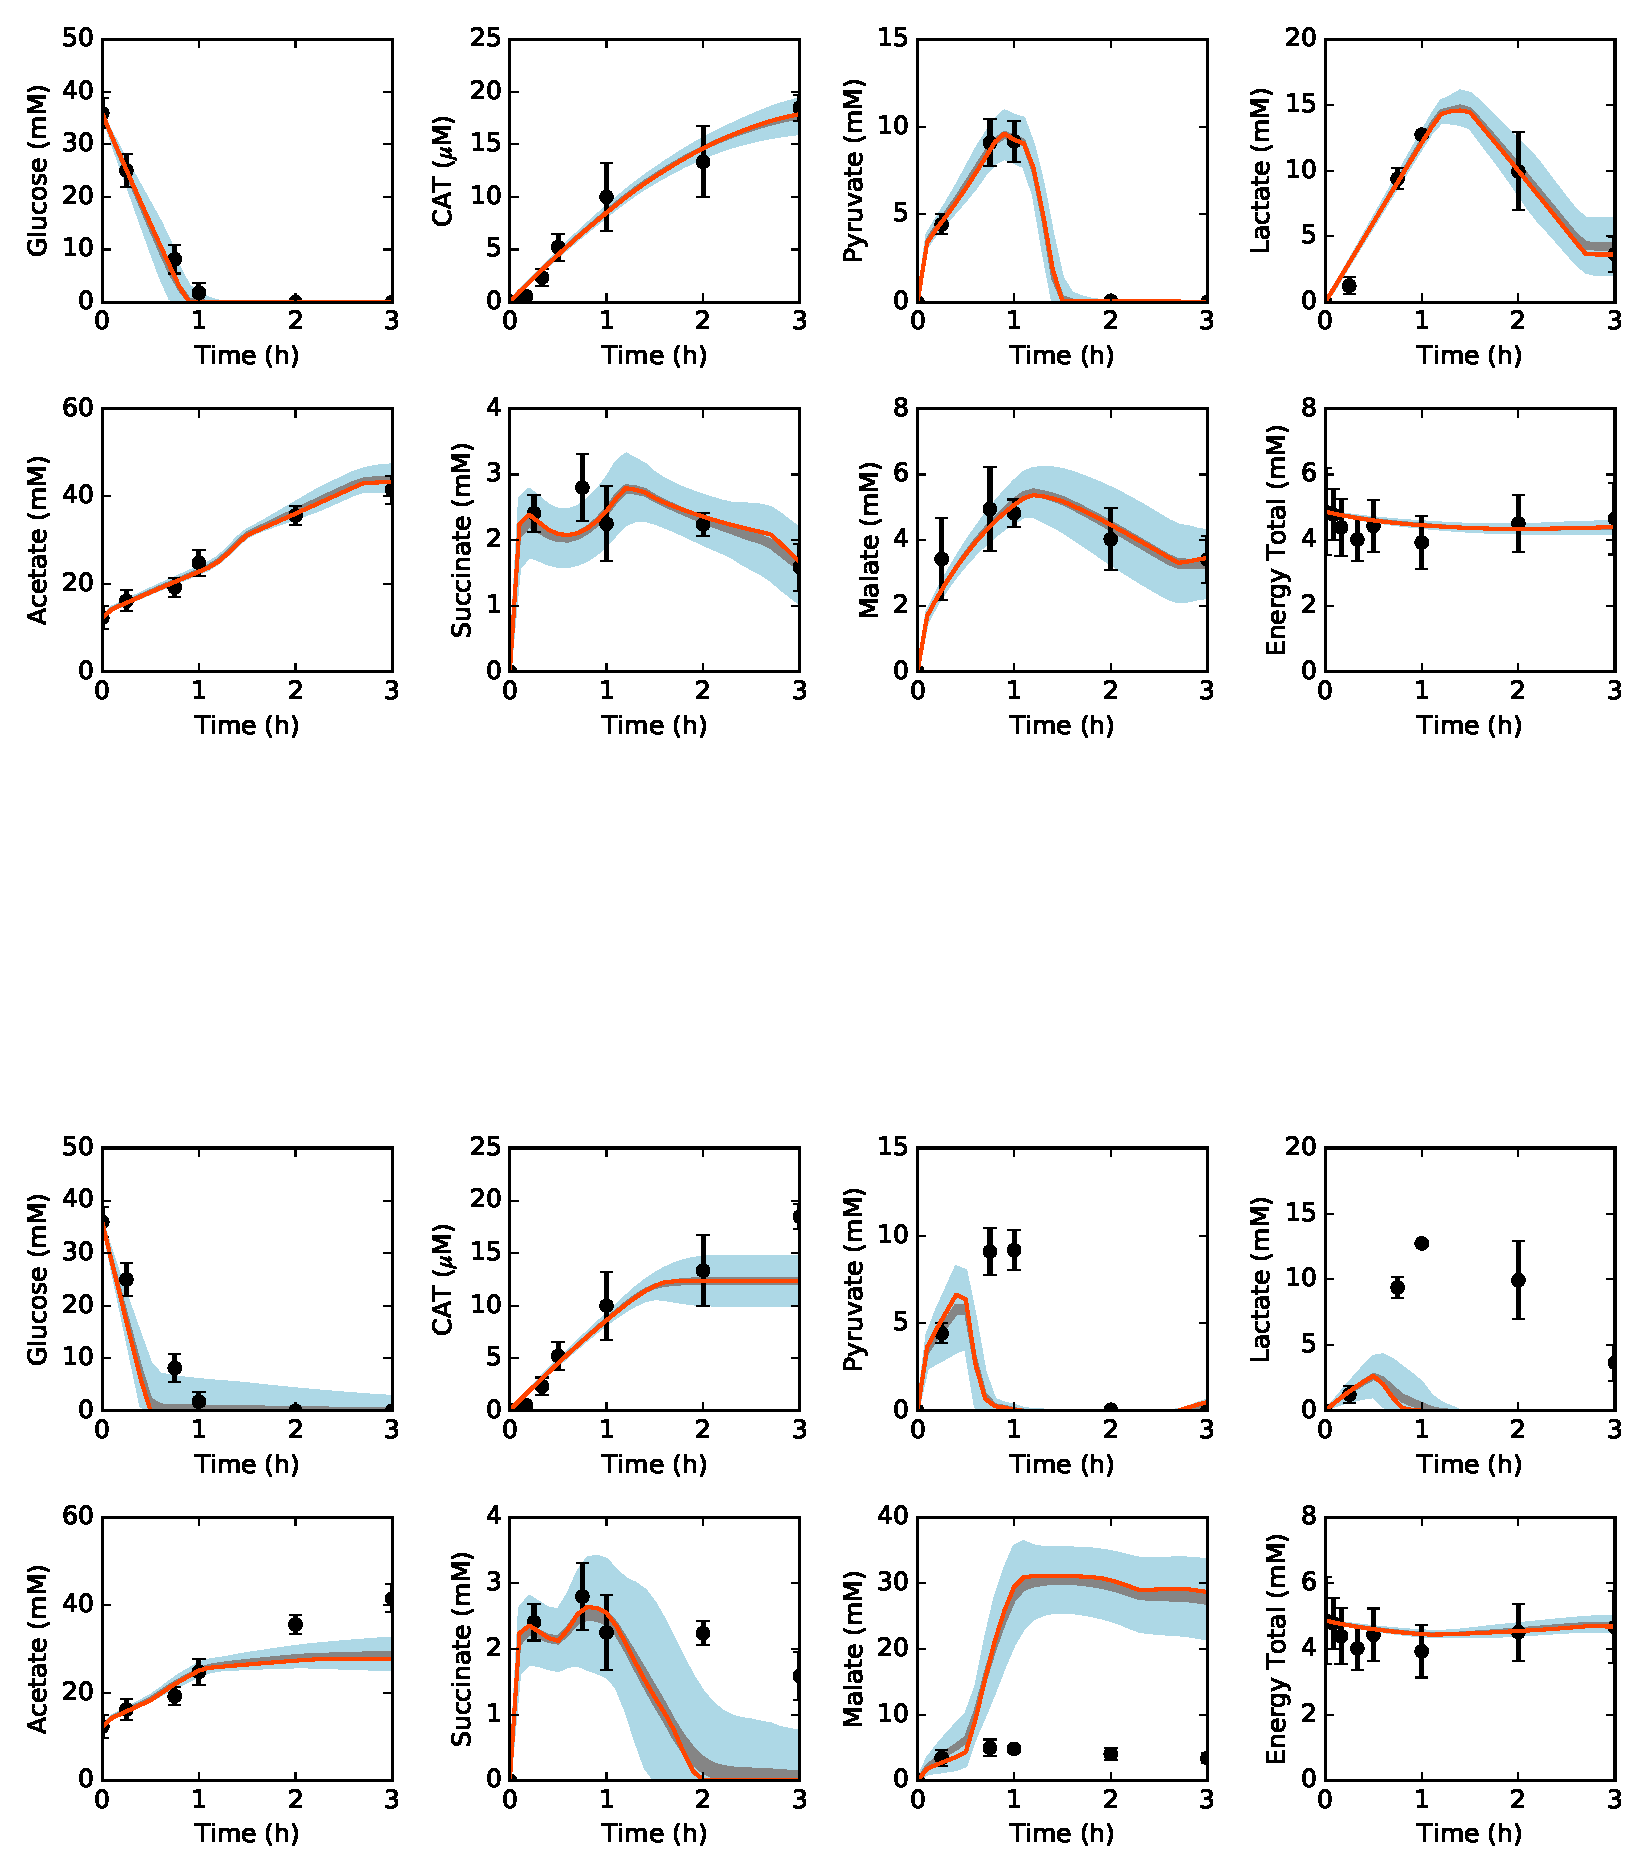
\includegraphics[width=1.00\textwidth]{./Figures/CarbonBoth.pdf}
% \caption{Central carbon metabolism in the presence (top) and absence (bottom) of allosteric control, including glucose (substrate), CAT (product), and intermediates, as well as total concentration of energy species. Best-fit parameter set (orange line) versus experimental data (points). 95\% confidence interval (blue shaded region) and 95\% confidence interval of the mean (gray shaded region) over the ensemble of 100 sets.}
% \label{fig:CarbonBoth}
% \end{figure}

\begin{figure}[ht]
\centering
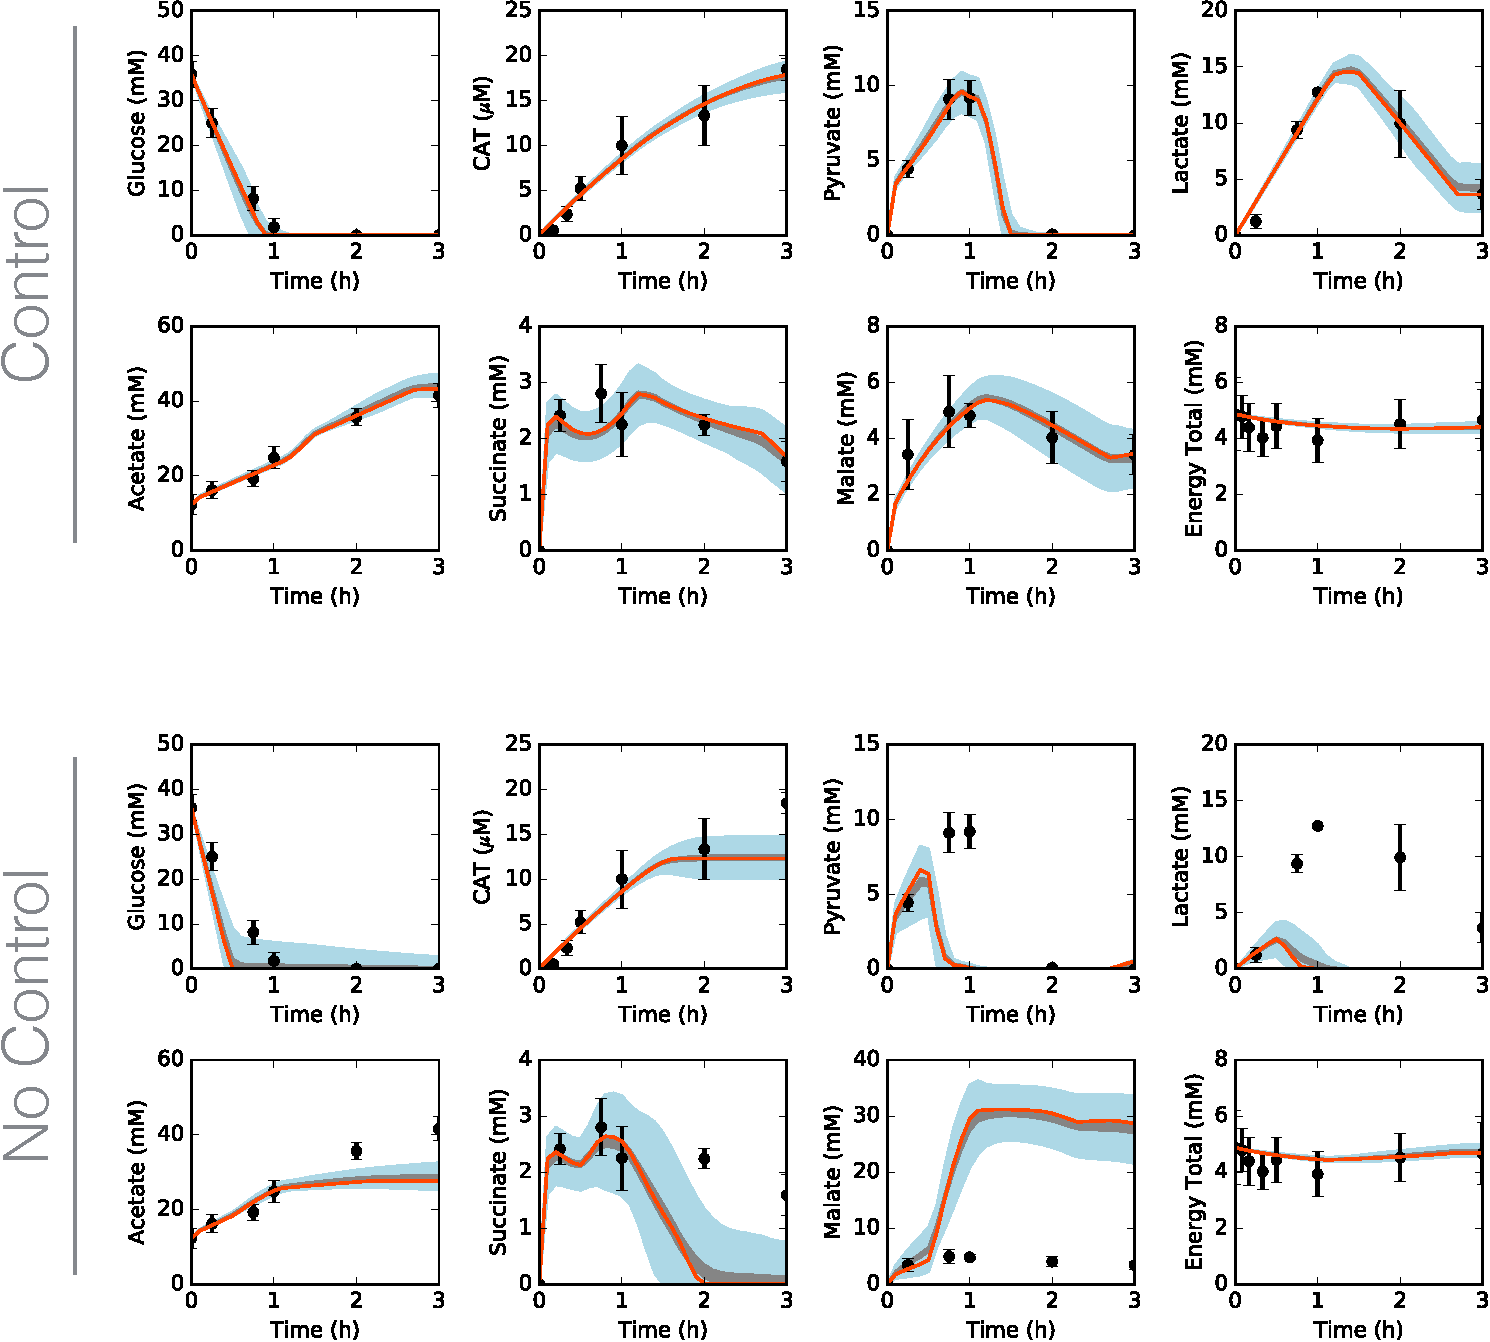
\includegraphics[width=1.00\textwidth]{./Figures/allostericControl_noindex.pdf}
\caption{Central carbon metabolism in the presence (top) and absence (bottom) of allosteric control, including glucose (substrate), CAT (product), and intermediates, as well as total concentration of energy species. Best-fit parameter set (orange line) versus experimental data (points). 95\% confidence interval (blue shaded region) and 95\% confidence interval of the mean (gray shaded region) over the ensemble of 100 sets.}
\label{fig:CarbonBoth}
\end{figure}

\begin{figure}[ht]
\centering
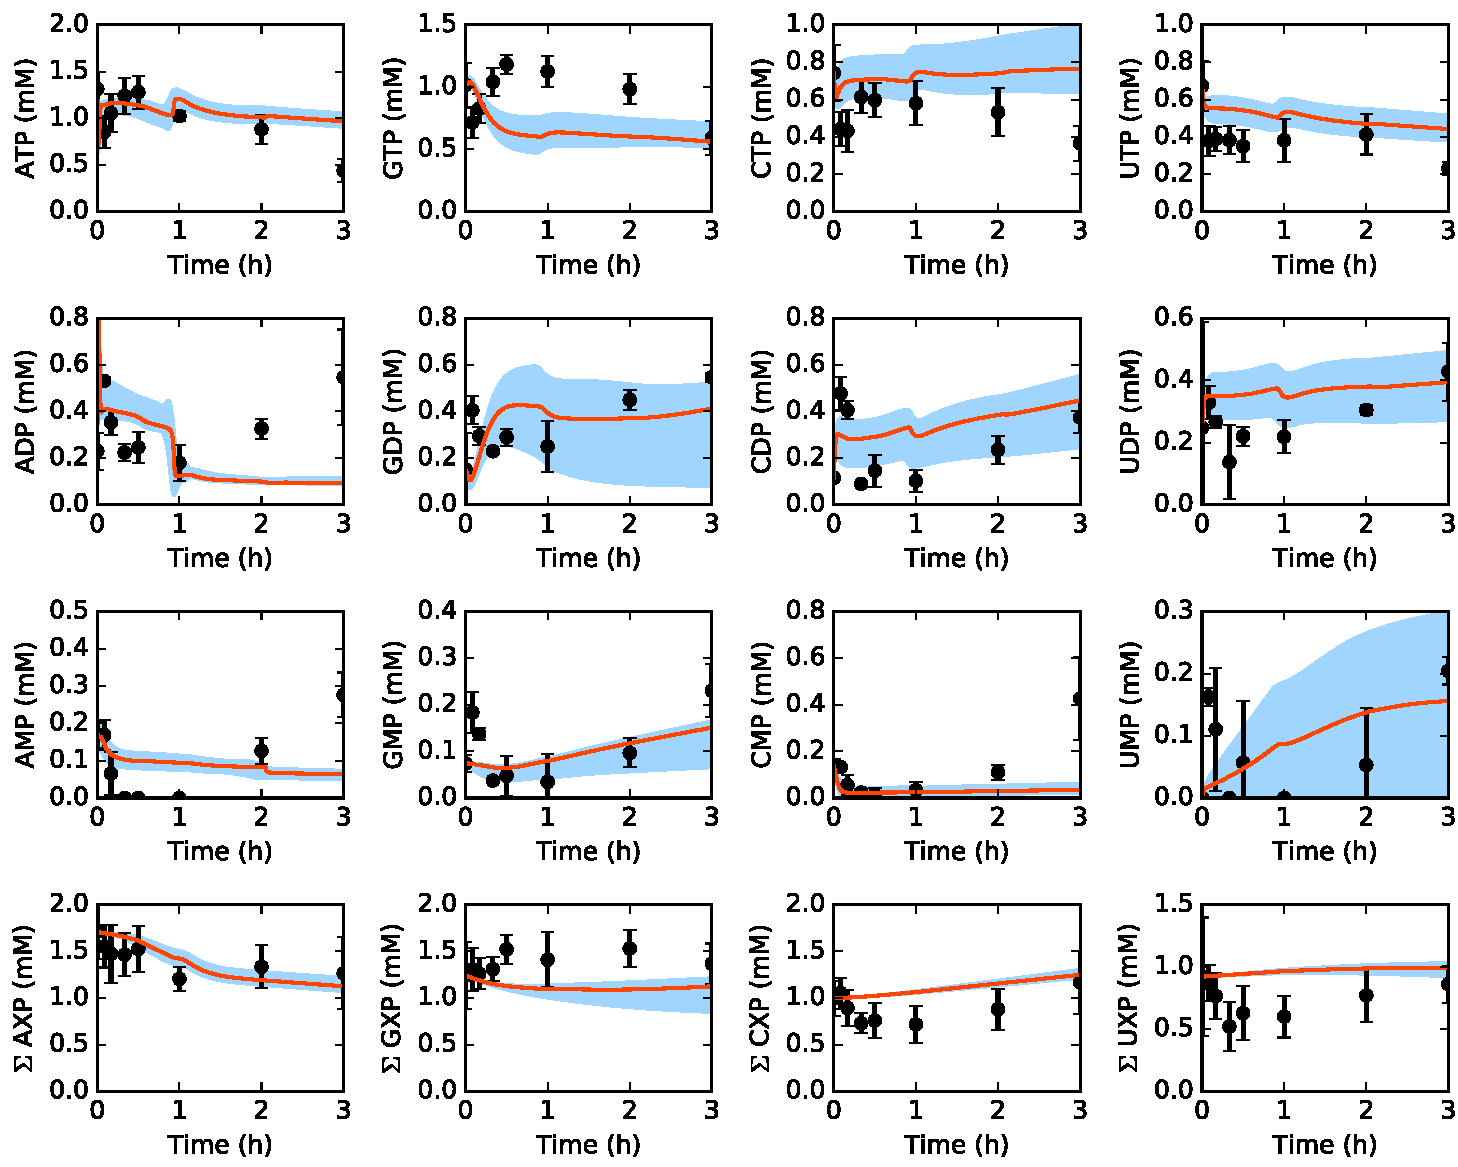
\includegraphics[width=1.00\textwidth]{./Figures/Energy.pdf}
\caption{Energy species and energy totals by base in the presence of allosteric control. Best-fit parameter set (orange line) versus experimental data (points). 95\% confidence interval (blue shaded region) and 95\% confidence interval of the mean (gray shaded region) over the ensemble of 100 sets.}
\label{fig:Energy}
\end{figure}

\begin{figure}[ht]
\centering
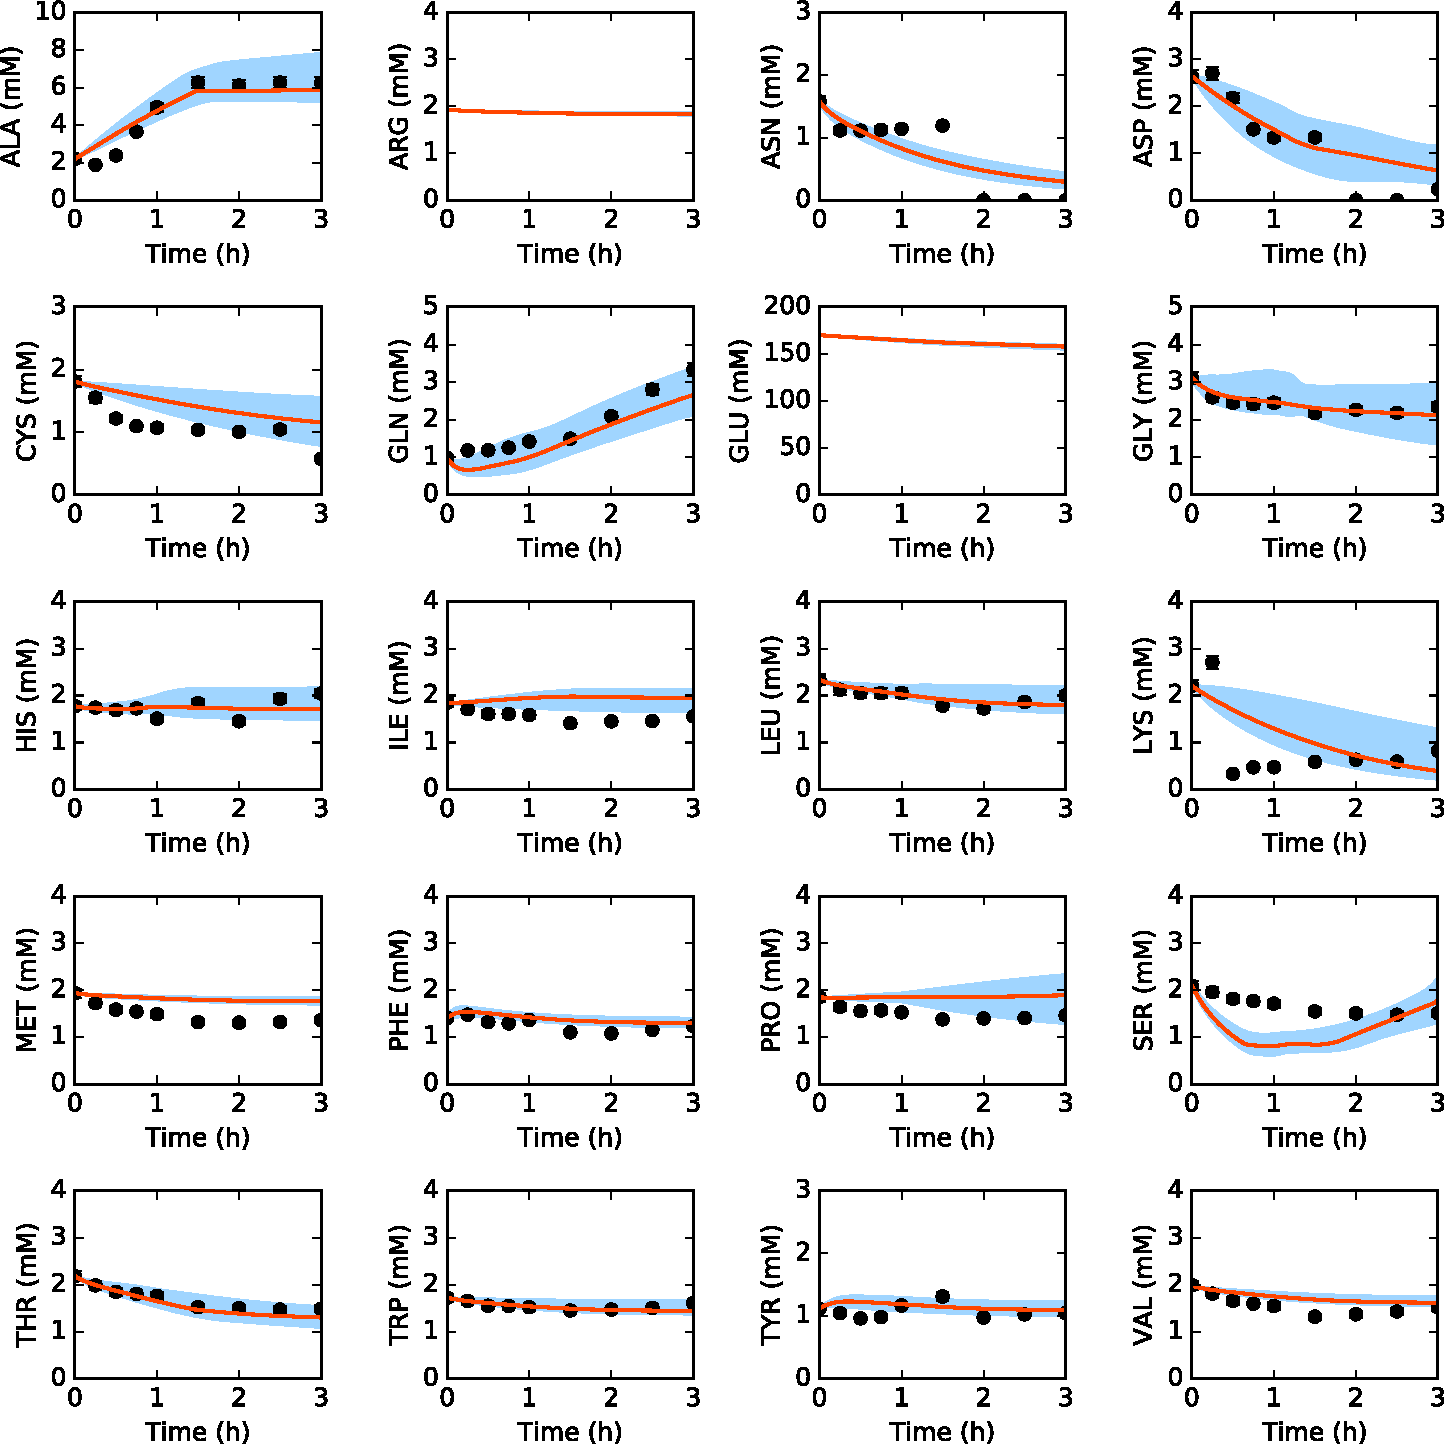
\includegraphics[width=1.00\textwidth]{./Figures/Amino.pdf}
\caption{Amino acids in the presence of allosteric control. Best-fit parameter set (orange line) versus experimental data (points). 95\% confidence interval (blue shaded region) and 95\% confidence interval of the mean (gray shaded region) over the ensemble of 100 sets.}
\label{fig:Amino}
\end{figure}

\begin{figure}[ht]
\centering
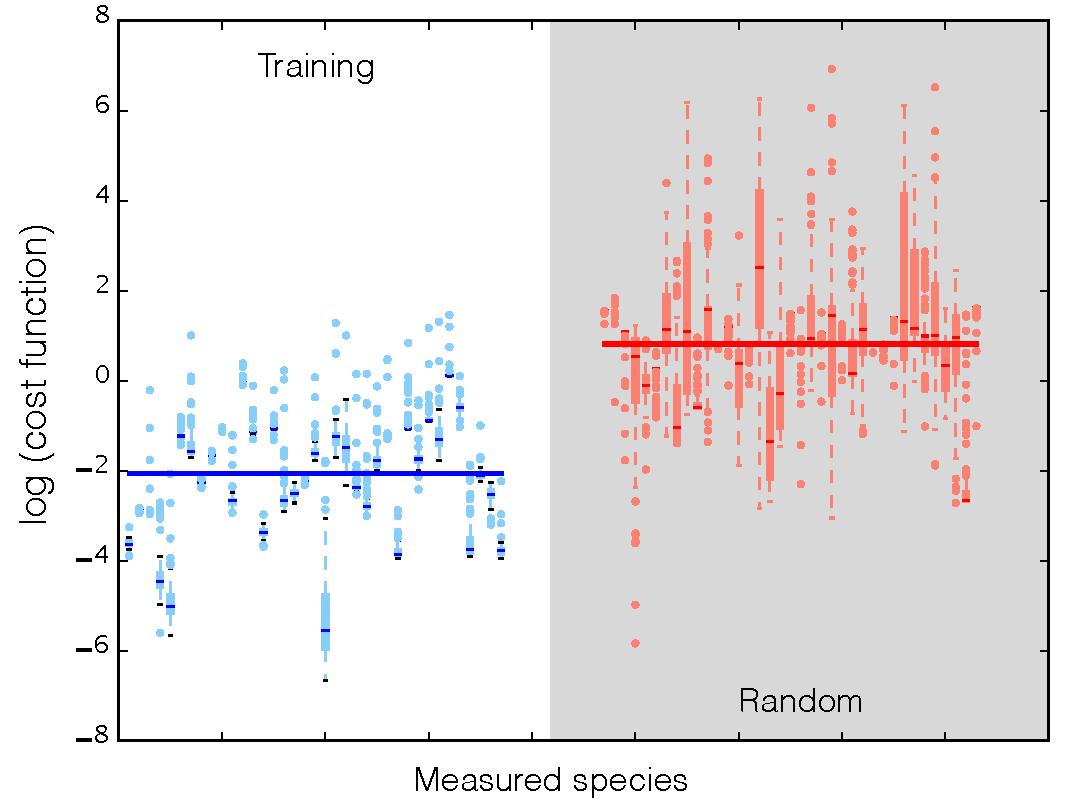
\includegraphics[width=1.00\textwidth]{./Figures/BoxPlot-KCFM.pdf}
\caption{Log of cost function across 37 datasets for data-trained ensemble (blue) and randomly generated ensemble (red, gray background). Median (bars), interquartile range (boxes), range excluding outliers (dashed lines), and outliers (circles) for each dataset. Median across all datasets (large bar overlaid).}
\label{fig:BoxPlot}
\end{figure}

\begin{figure}[ht]
\centering
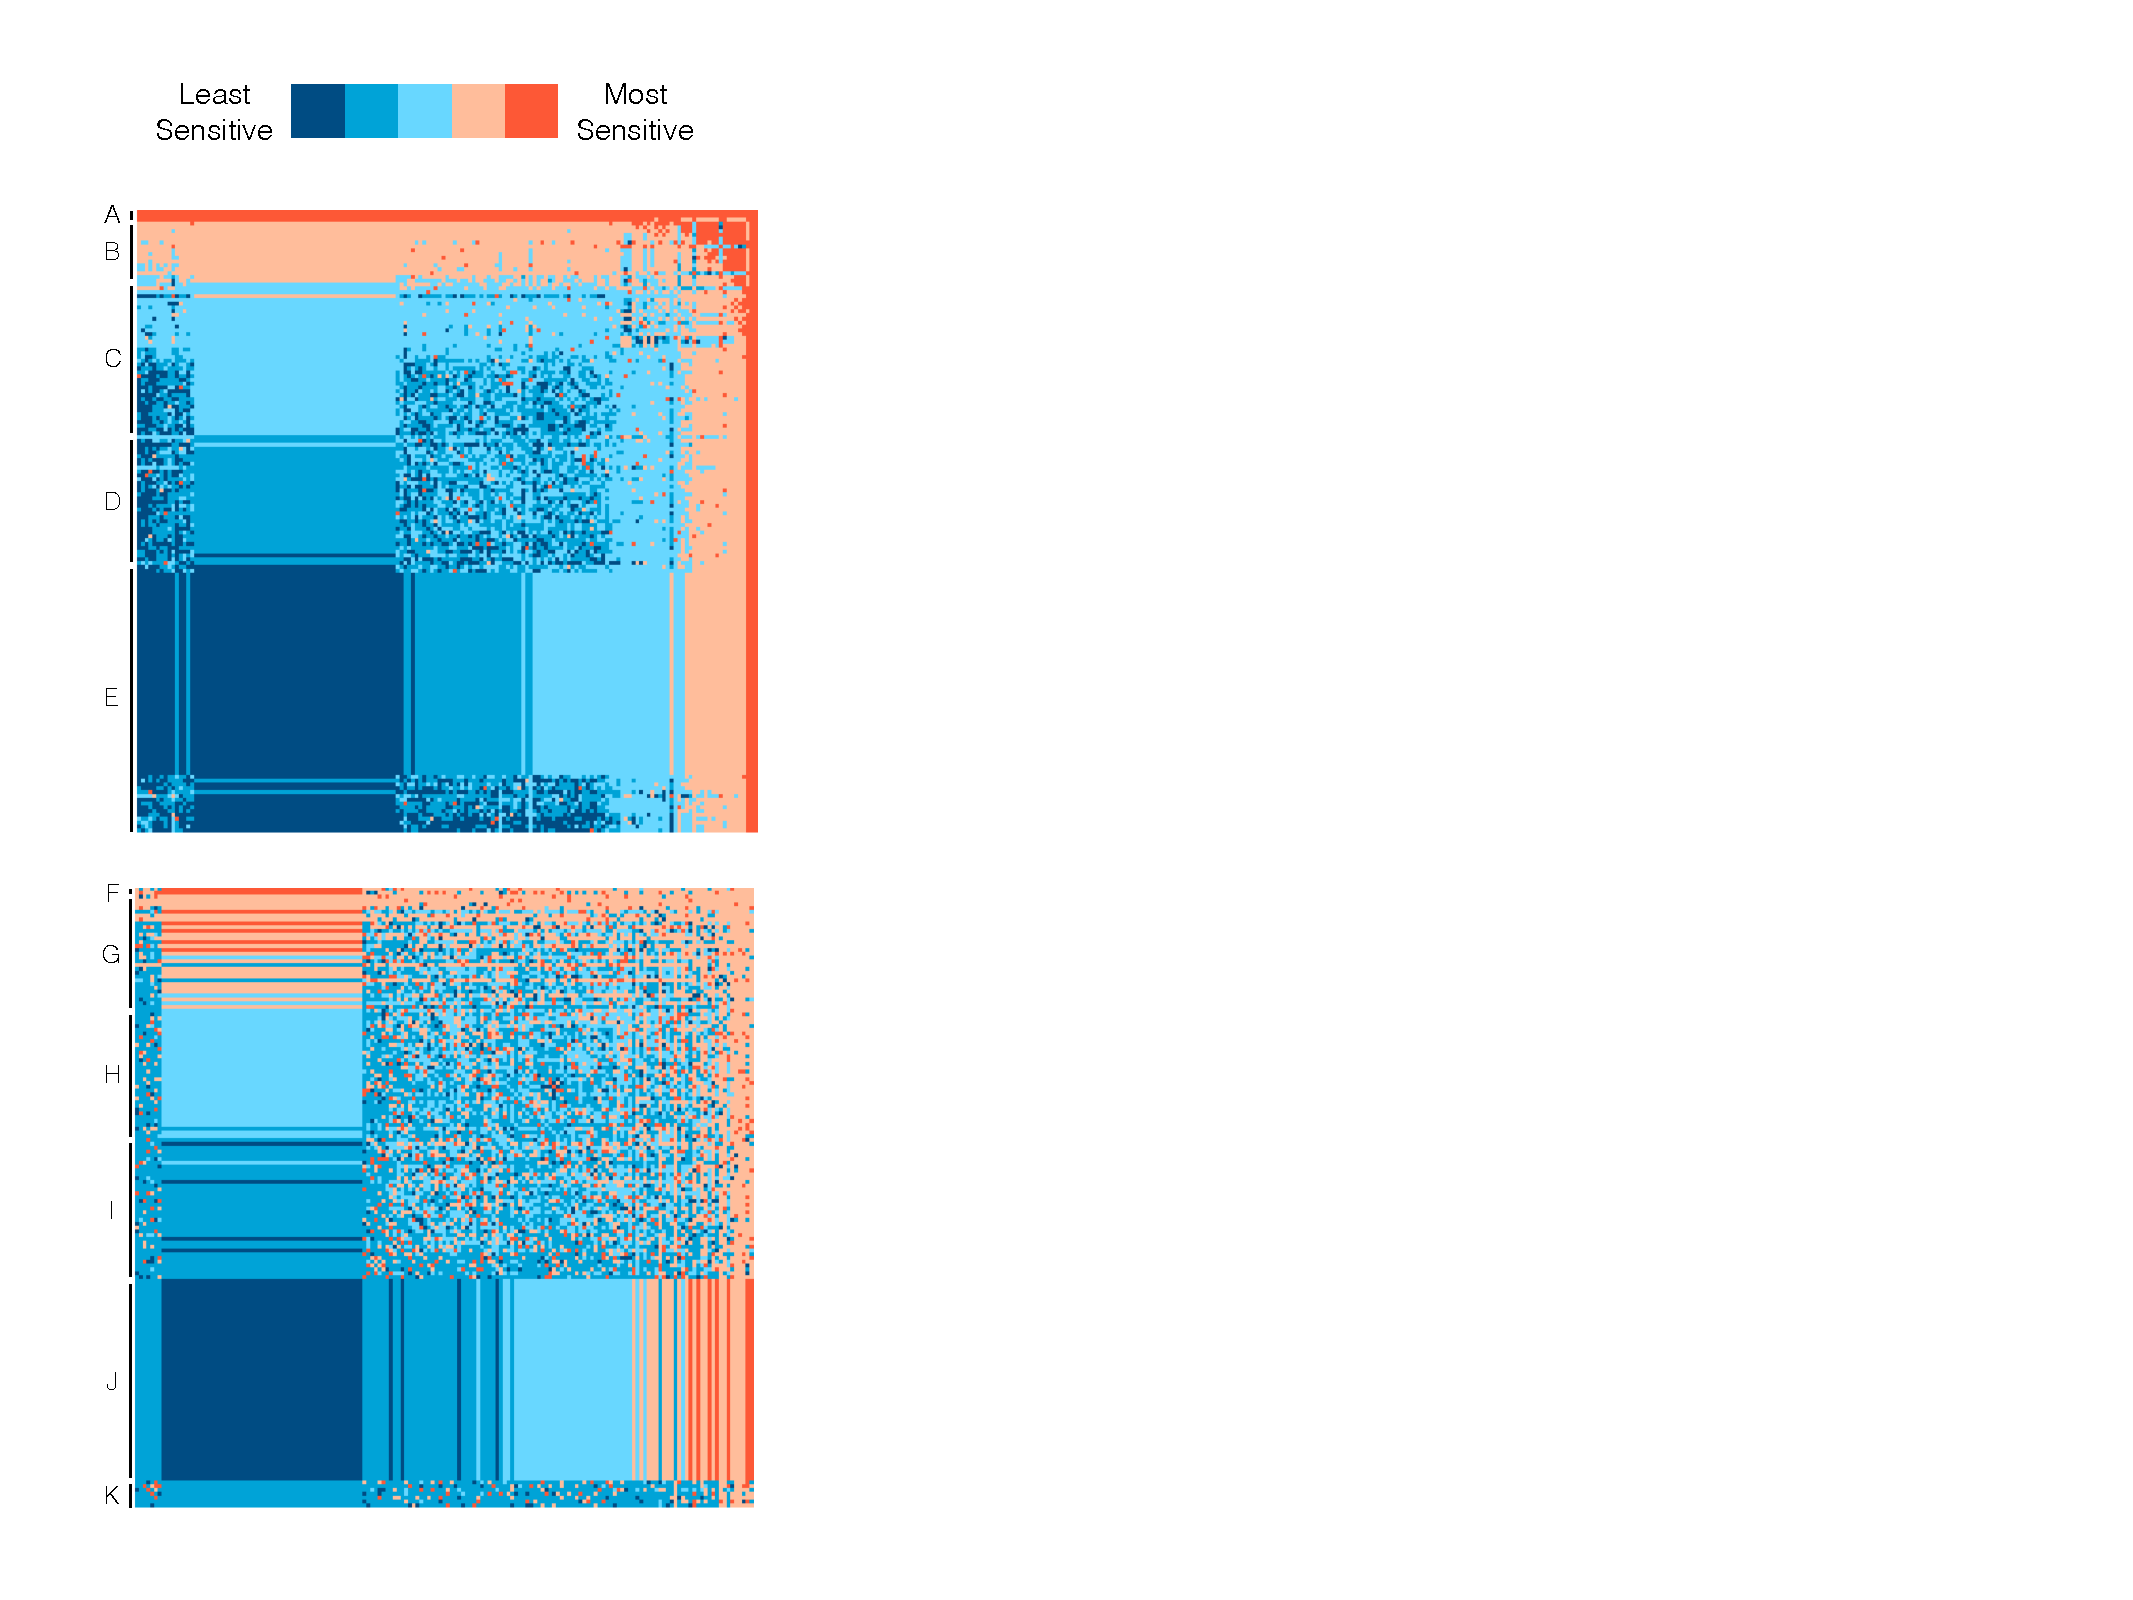
\includegraphics[width=0.76\textwidth,trim=0 28 615 40,clip]{./Figures/Sensitivity.pdf}
\caption{Normalized first-order and pairwise sensitivities of CAT production (top) and system state (bottom) to maximum reaction rates.}
\label{fig:Sensitivity}
\end{figure}

%\begin{figure}[ht]
%\centering
%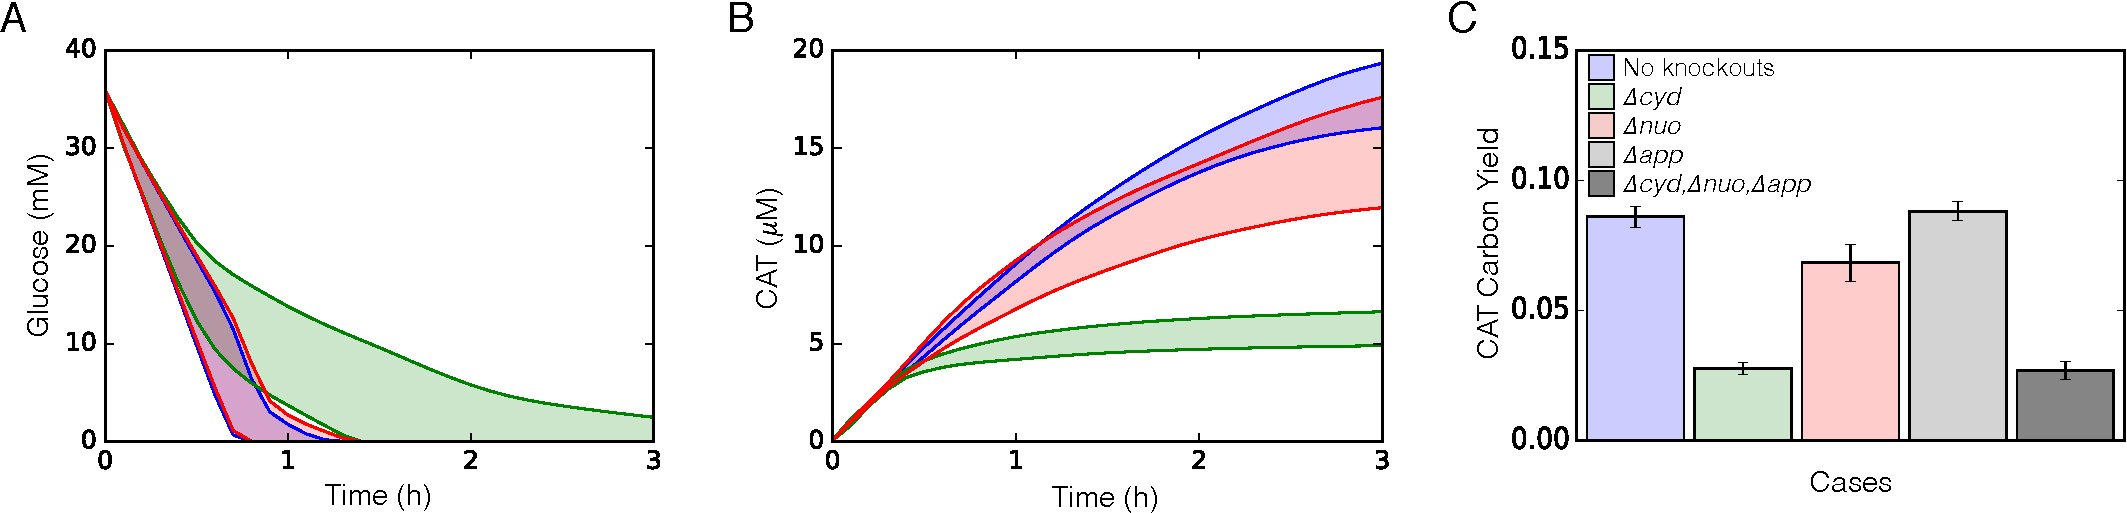
\includegraphics[width=1\textwidth]{./Figures/oxphos_ko.pdf}
%\caption{The effect of oxidative phosphorylation on glucose uptake, CAT production and CAT carbon yield. A. 95\% confidence interval of an ensemble for glucose concentration versus time for no knockouts (blue shaded region), \textit{cyd} knockout (green shaded region), and \textit{nuo} knockout (red shaded region). B. 95\% confidence interval of an ensemble for CAT concentration versus time for no knockouts (blue shaded region), \textit{cyd} knockout (green shaded region), and \textit{nuo} knockout (red shaded region). C. CAT carbon yield for 5 different cases of oxidative phosphorylation: no knockouts (blue), \textit{cyd} knockout (green), \textit{nuo} knockout (red), \textit{app} knockout (light gray), and a combination of \textit{cyd}, \textit{nuo}, \textit{app} knockouts (dark gray).}
%\label{fig:oxphos_ko}
%\end{figure}
%\clearpage

%\begin{figure}[ht]
%\centering
%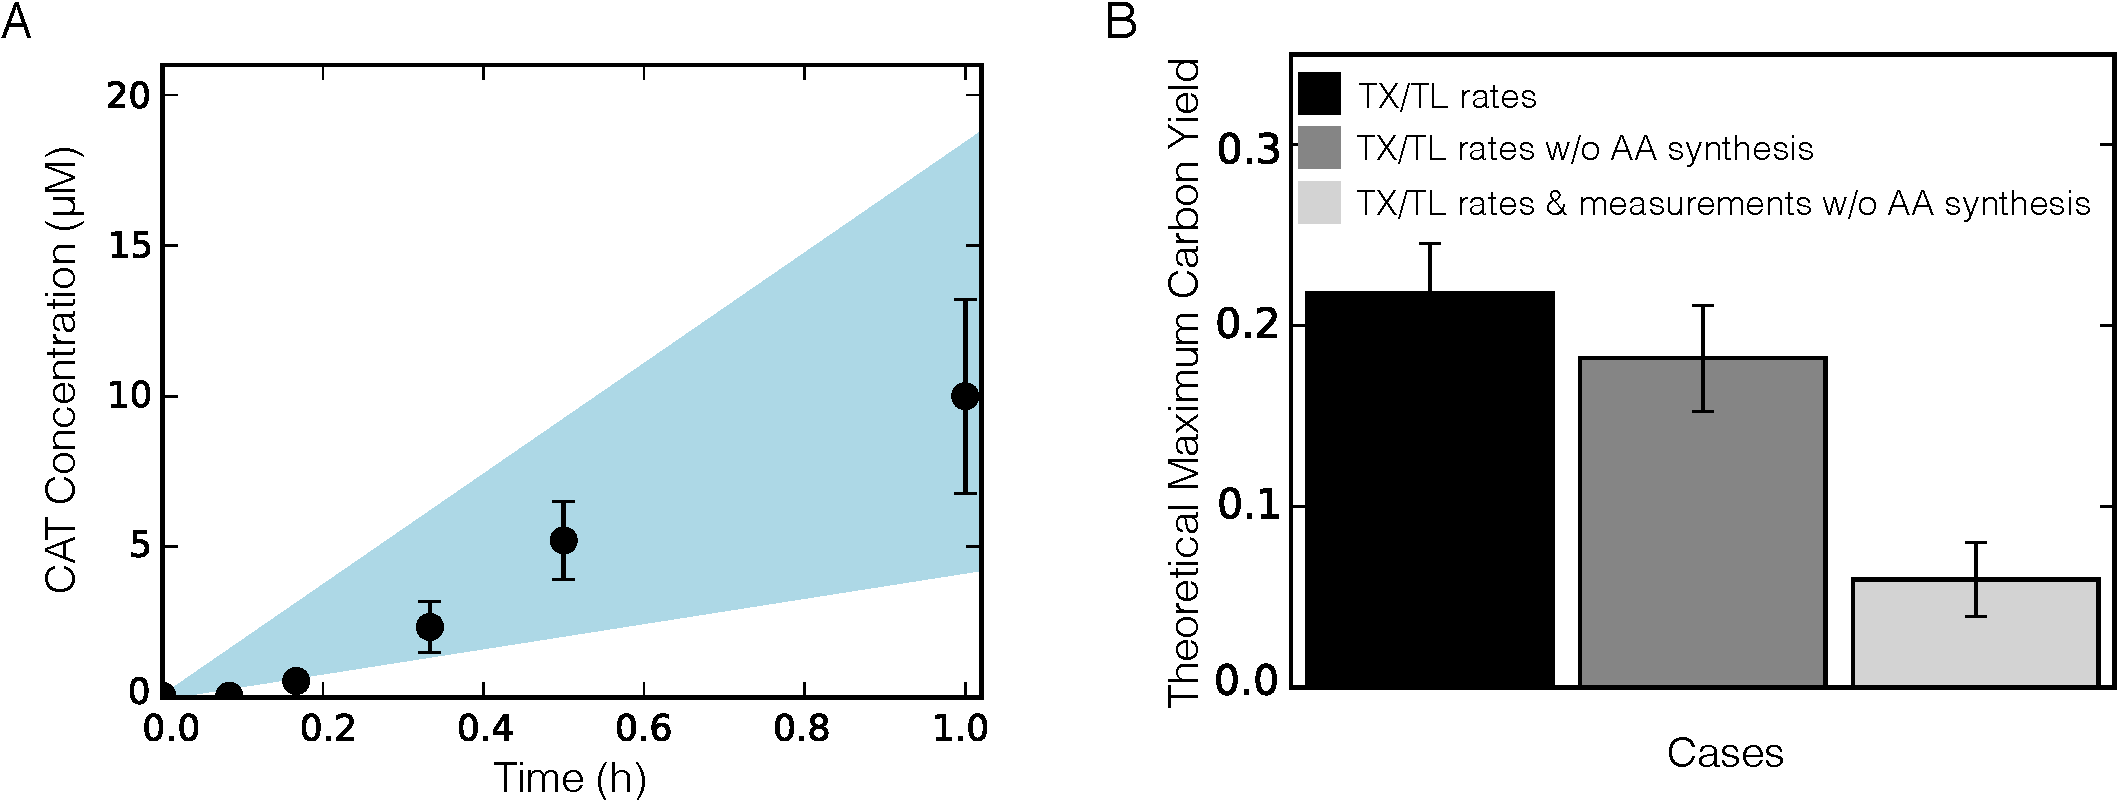
\includegraphics[width=1\textwidth]{./Figures/CAT_prod_yield.pdf}
%\caption{Sequence-specific flux balance analysis of CAT production and yield. A. 95\% confidence interval of the ensemble (light blue region) for CAT concentration versus time. B. Theoretical maximum carbon yield of CAT calcualted by ssFBA for three different cases: constrained by transcription/translation (TX/TL) rates (black), same as previous but without amino acid synthesis reactions (gray), and same as previous but constrained by experimental measurements where available (light gray). Error bars represent standard deviation of the ensemble.}
%\label{fig:CATProdYield}
%\end{figure}
%\clearpage

\begin{figure}[ht]
\centering
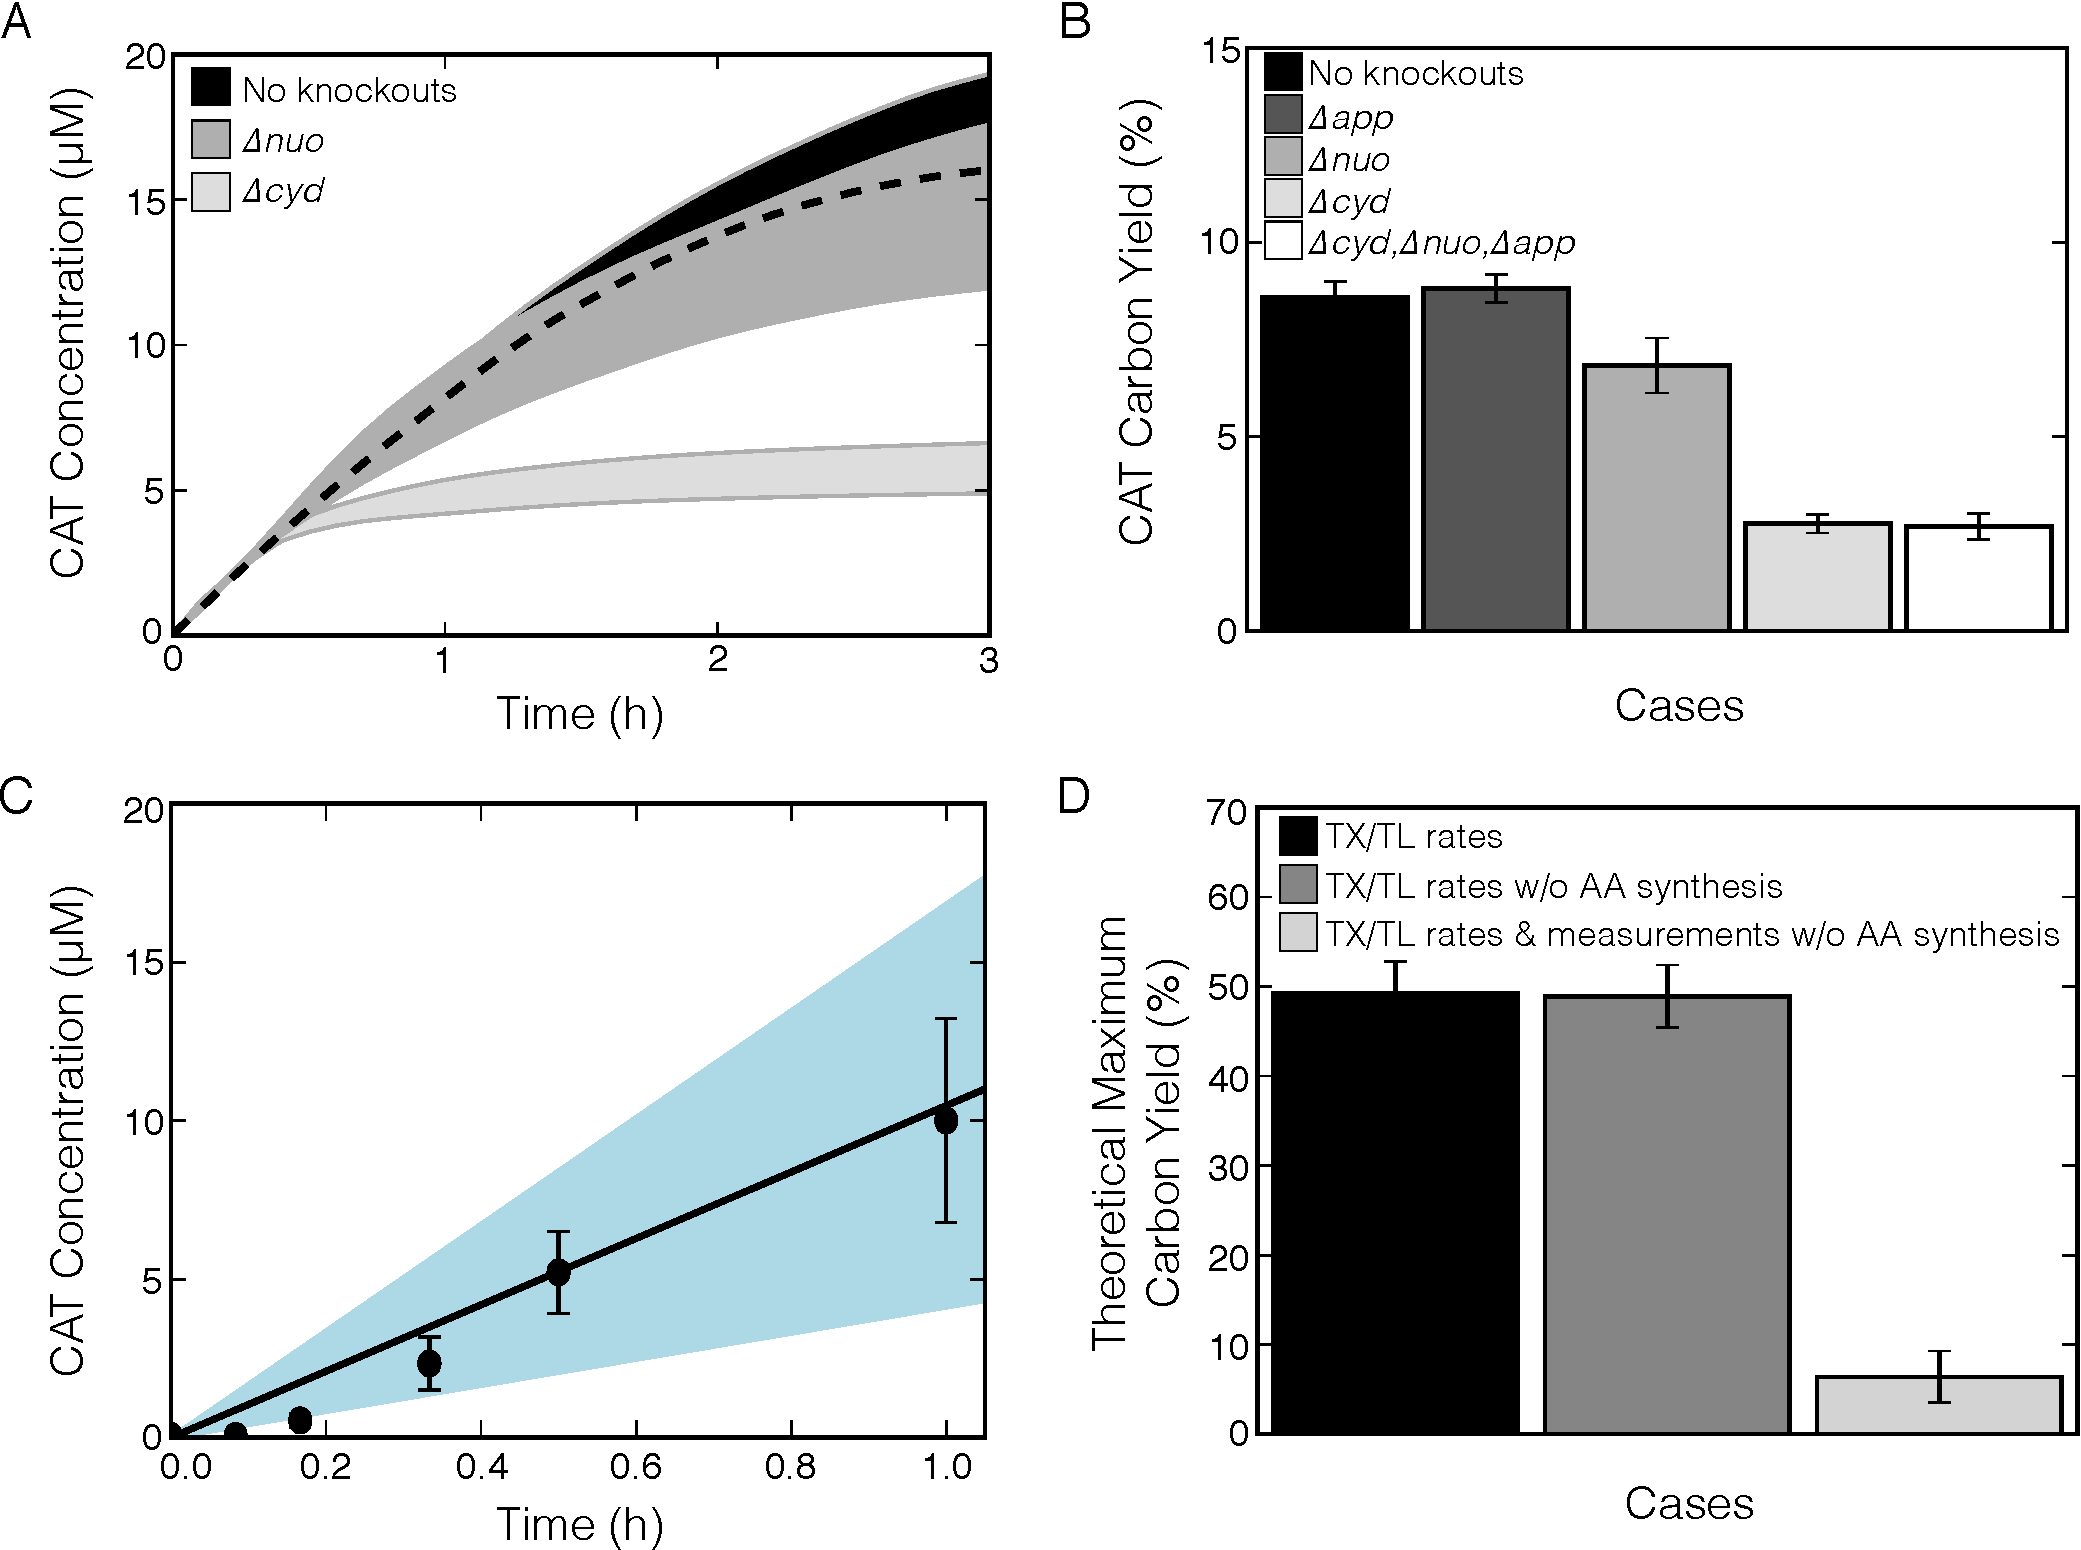
\includegraphics[width=1\textwidth]{./Figures/oxKO_ssFBA_yields.pdf}
\caption{The effects of oxidative phosphorylation and amino acid synthesis pathways on CAT production and carbon yield. A. 95\% confidence interval of the ensemble of kinetic models for CAT concentration versus time, for the best-fit set with no knockouts (black shaded region and dashed line), \textit{nuo} knockout (medium gray), and \textit{cyd} knockout (light gray). B. CAT carbon yield of the ensemble of kinetic models for no knockouts (black), \textit{app} knockout (dark gray), \textit{nuo} knockout (medium gray), \textit{cyd} knockout (light gray), and all three knockouts (white). Error bars represent standard deviation of the ensemble. C. 95\% confidence interval of the ensemble of ssFBA simulations (light blue region) of CAT concentration over time, against experimental data (black). D. Theoretical maximum carbon yield of CAT production, calcualted by ssFBA for three different cases: constrained by transcription/translation (TX/TL) rates (black), same as previous but without amino acid synthesis reactions (medium gray), and same as previous but constrained by experimental measurements where available (light gray). Error bars represent standard deviation of the ensemble.}
\label{fig:oxKO_ssFBA_yields}
\end{figure}
\clearpage

\begin{figure}[ht]
\centering
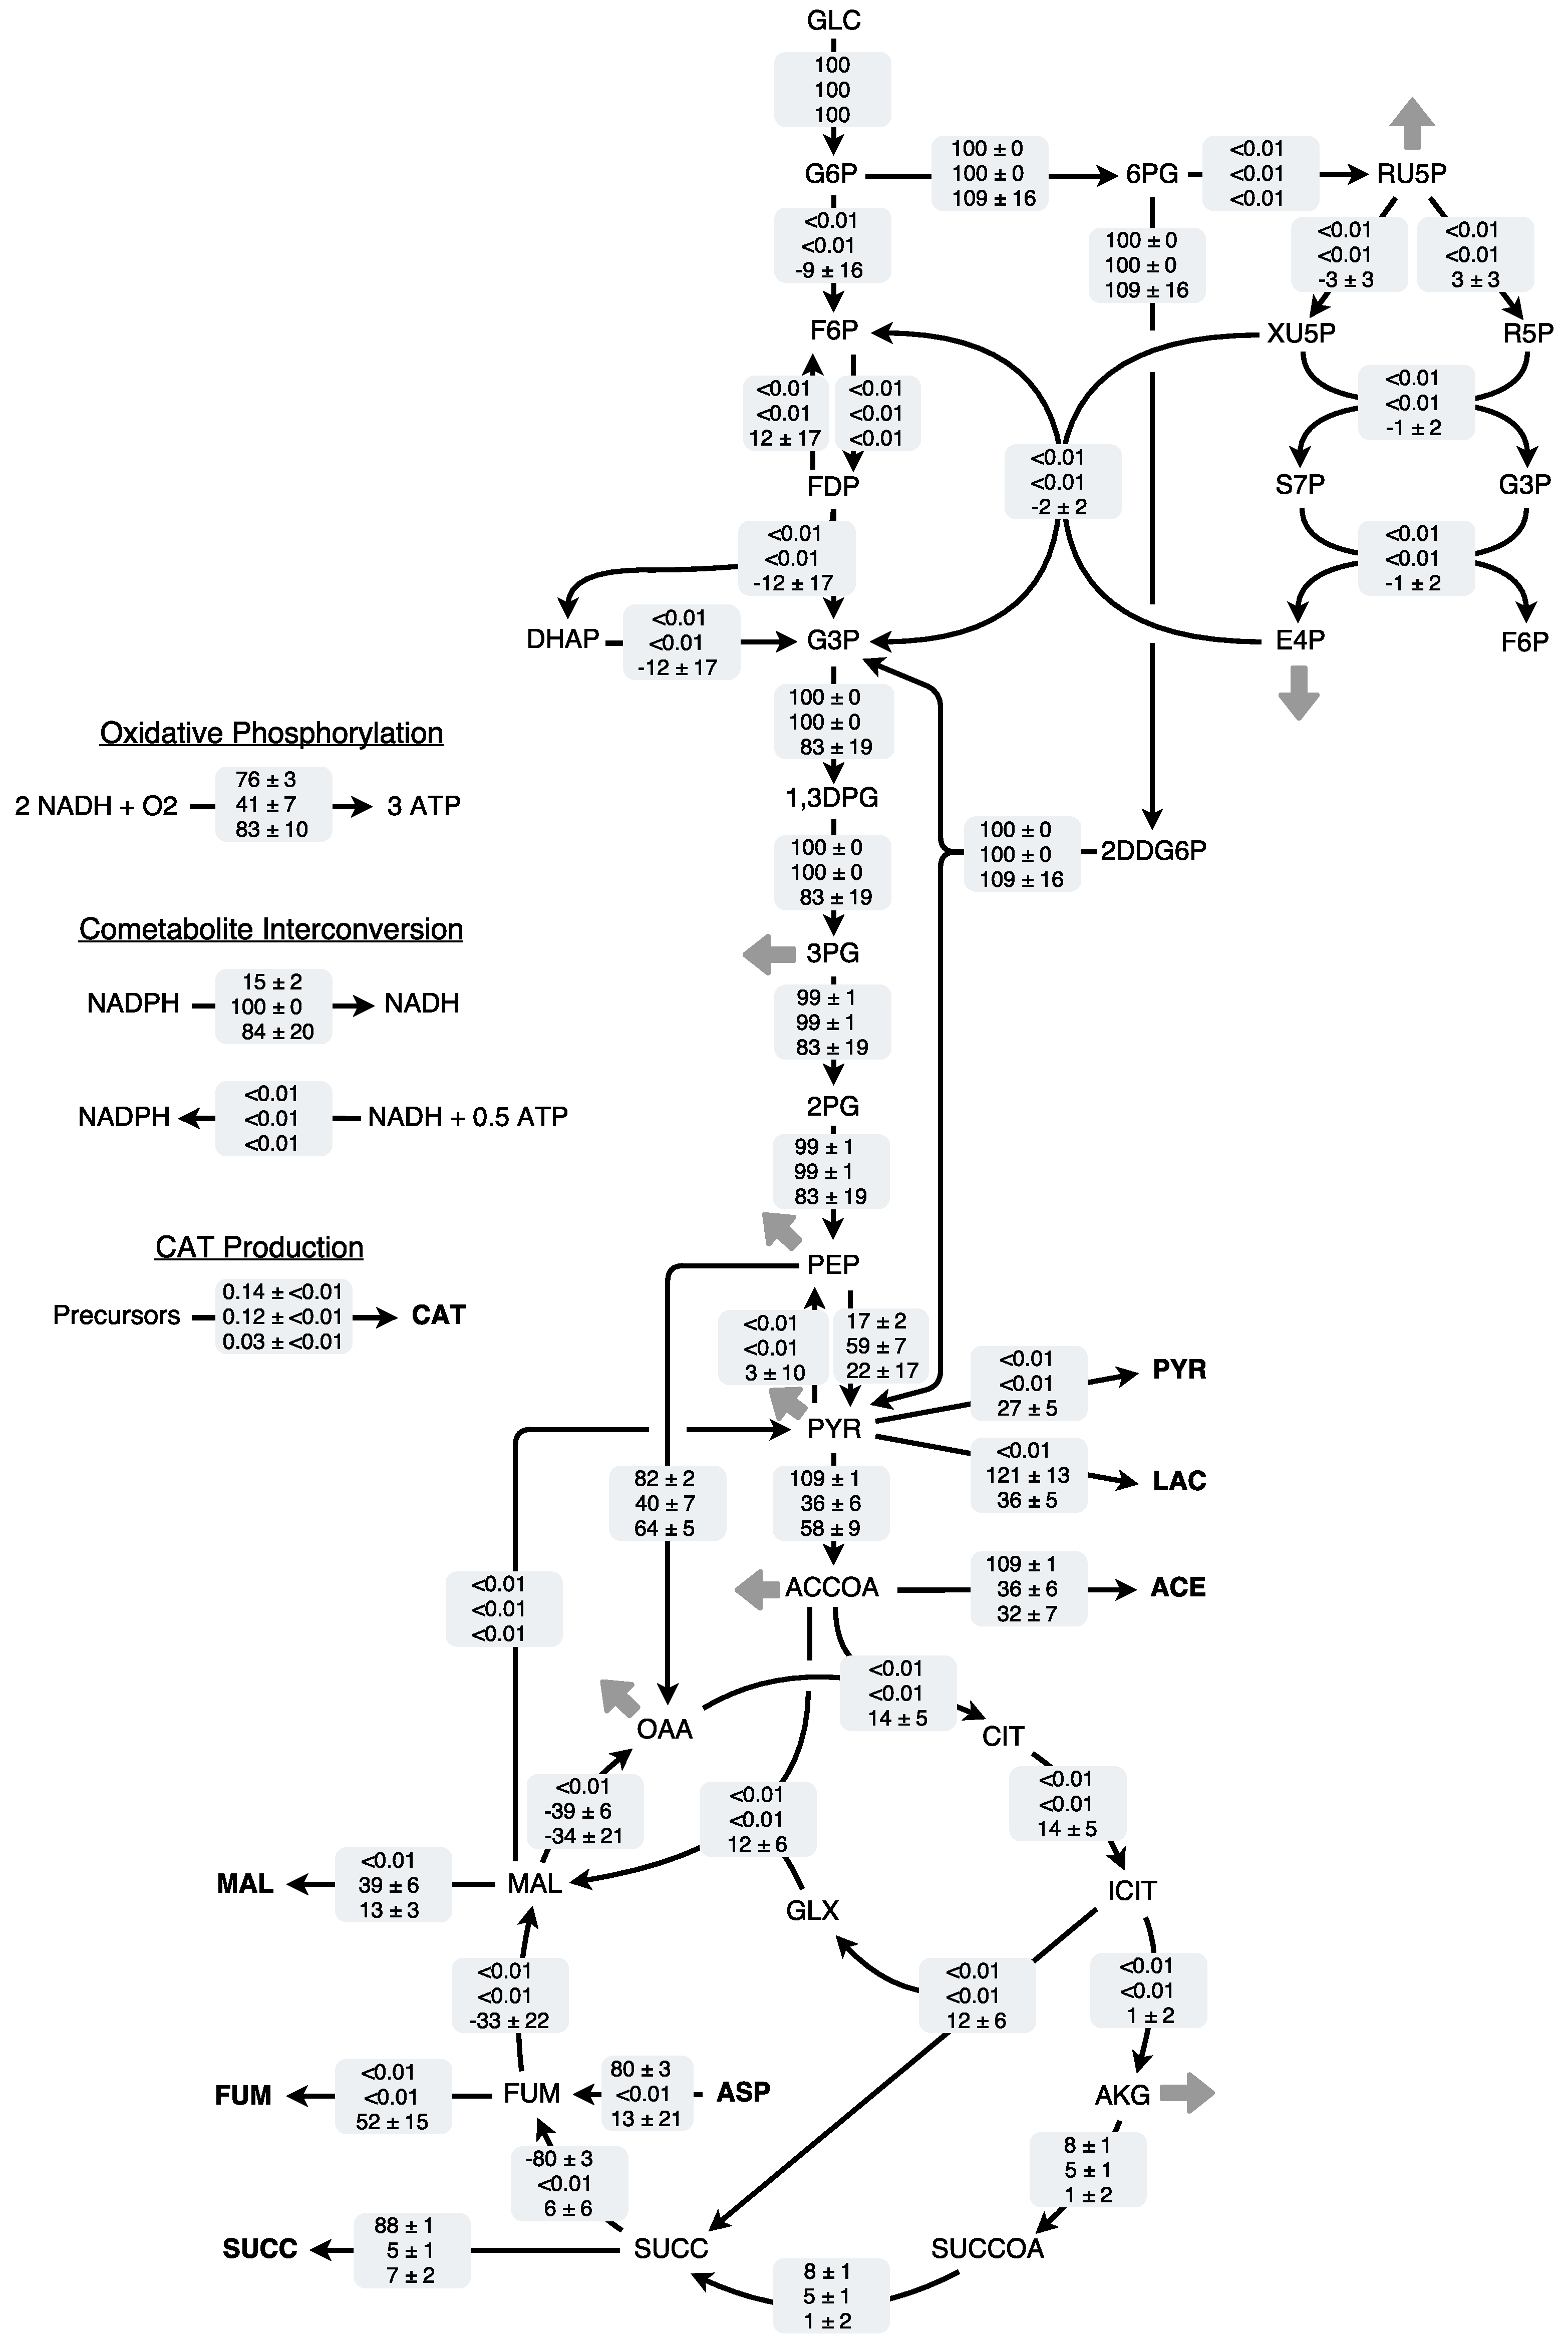
\includegraphics[width=0.75\textwidth]{./Figures/CAT_flux_final.pdf}
\caption{Flux profile for glycolysis, pentose phosphate pathway, Entner-Doudoroff pathway, TCA cycle, NADPH/NADH transfer, and oxidative phosphorylation. Sequence-specific FBA flux value (mean ± standard deviation) across ensemble for 1 hr, normalized to glucose uptake flux. Flux distribution for three different cases: constrained by transcription and translation rates (top row), same as previous but without amino acid synthesis reactions  (second row), and same as previous but constrained by experimental measurements where available (bottom row).}
\label{fig:Network}
\end{figure}

\begin{table}
\centering
    \caption{CAT carbon yield breakdown for best-fit set, knockouts, and experimental data. Carbon produced as CAT, carbon consumed as glucose and each amino acid, sum of consumed species, and yield.}
    \renewcommand{\arraystretch}{1.3}
    \begin{tabular}{lrrrrrr} \toprule
        Carbon Produced (C-mM) & Best-fit & $\Delta$cyd & $\Delta$nuo & $\Delta$app & \parbox{1 cm}{$\Delta$cyd $\Delta$nuo $\Delta$app} & Data \\ \hline
        CAT & 20.9 & 6.5 & 18.1 & 21.4 & 5.1 & 21.6 \\ \midrule
        Carbon Consumed (C-mM) \\ \hline
        GLC & 215.4 & 215.4 & 215.4 & 215.4 & 159.8 & 215.4 \\ \hline
        ALA & 0.0 & 0.0 & 1.7 & 0.0 & 0.0 & 0.0 \\ \hline
%        ARG & 10.2 & 0.9 & 1.1 & 9.9 & 1.3 & - \\ \hline
        ASN & 6.2 & 6.3 & 6.2 & 6.2 & 6.3 & 6.3 \\ \hline
        ASP & 7.5 & 0.0 & 3.9 & 7.5 & 0.0 & 9.6 \\ \hline
        CYS & 3.0 & 2.9 & 3.0 & 3.1 & 2.9 & 3.7 \\ \hline
        GLN & 0.0 & 1.8 & 0.0 & 0.0 & 2.7 & 0.0 \\ \hline
%        GLU & 492.6 & 505.1 & 528.2 & 505.6 & 501.8 & - \\ \hline
        GLY & 3.1 & 1.1 & 2.6 & 3.1 & 0.9 & 1.5 \\ \hline
        HIS & 0.2 & 0.4 & 1.1 & 0.2 & 0.3 & 0.0 \\ \hline
        ILE & 1.0 & 0.3 & 0.8 & 1.0 & 0.2 & 1.7 \\ \hline
        LEU & 1.4 & 0.4 & 1.2 & 1.4 & 0.3 & 2 \\ \hline
        LYS & 10.7 & 13.2 & 13.1 & 10.7 & 13.2 & 8.3 \\ \hline
        MET & 0.8 & 0.2 & 0.7 & 0.8 & 0.2 & 2.9 \\ \hline
        PHE & 3.2 & 1.0 & 2.8 & 3.3 & 0.8 & 1.6 \\ \hline
        PRO & 2.4 & 0.2 & 0.7 & 2.4 & 0.2 & 1.9 \\ \hline
        SER & 2.5 & 2.1 & 2.4 & 2.5 & 2.1 & 1.8 \\ \hline
        THR & 3.4 & 2.9 & 3.3 & 3.4 & 2.8 & 2.8 \\ \hline
        TRP & 1.0 & 0.3 & 0.8 & 1.0 & 0.2 & 1.2 \\ \hline
        TYR & 1.1 & 0.4 & 1.1 & 1.1 & 0.4 & 0.6 \\ \hline
        VAL & 1.4 & 0.4 & 1.2 & 1.5 & 0.4 & 2.4 \\ \midrule
%        Sum & 767.1 & 755.3 & 791.3 & 780.1 & 696.8 & - \\ \hline
        Sum & 264.3 & 249.3 & 262.0 & 264.6 & 193.7 & 263.7 \\ \midrule
%        Yield & 2.7\% & 0.9\% & 2.3\% & 2.7\% & 0.7\% & - \\ \hline
        Yield & 7.9\% & 2.6\% & 6.9\% & 8.1\% & 2.7\% & 8.2\% \\ \bottomrule
    \end{tabular}
\label{tbl:yield_breakdown}
\end{table}

\begin{figure}[ht]
\centering
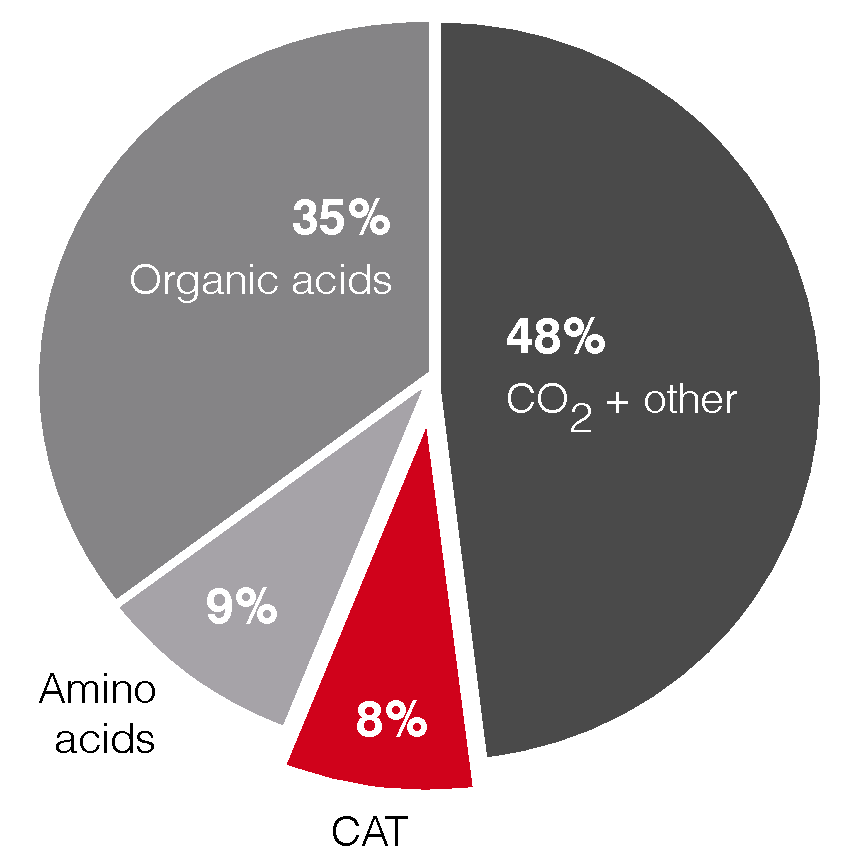
\includegraphics[width=0.75\textwidth]{./Figures/Carbon-Balance-BFS.pdf}
\caption{Carbon balance for the best-fit set. Carbon moles produced as CAT, amino acids (alanine and glutamine), organic acids (lactate, acetate, succinate, and malate), and other byproducts including carbon dioxide, as percentages of total carbon consumption (glucose and all other amino acids).}
\label{fig:Carbon_Balance}
\end{figure}

%\begin{table}
%\centering
%    \caption{Amino acid total net consumption, consumption toward CAT, and net consumption other than toward CAT for the best-fit set. Total net consumption defined as decrease in amino acid concentration over 3 hours. Consumption toward CAT defined as increase in CAT concentration over 3 hours, multiplied by stoichiometric coefficient for given amino acid in CAT synthesis.}
%    \renewcommand{\arraystretch}{1.3}
%    \begin{tabular}{lrrr} \toprule
%        & \parbox{3.6cm}{Total Net \phantom{abcdefgh} Consumption (mM)} & \parbox{3.4cm}{Consumption \phantom{abc} Toward CAT (mM)} & \parbox{3.6cm}{Other \phantom{abcdefgh} Consumption (mM)} \\ \hline
%        ALA  & -3.85 & 0.27 & -4.12 \\ \hline
%        ARG  & 1.70  & 0.18  & 1.52 \\ \hline
%        ASN  & 1.55  & 0.09  & 1.46 \\ \hline
%        ASP  & 1.87  & 0.21  & 1.66 \\ \hline
%        CYS  & 1.02  & 0.09  & 0.93 \\ \hline
%        GLN  & -2.28 & 0.21 & -2.49 \\ \hline
%        GLU  & 98.53  & 0.23  & 98.30 \\ \hline
%        GLY  & 1.55  & 0.18  & 1.37 \\ \hline
%        HIS  & 0.04  & 0.21  & -0.17 \\ \hline
%        ILE  & 0.16  & 0.16  & 0.00 \\ \hline
%        LEU  & 0.23  & 0.23  & 0.00 \\ \hline
%        LYS  & 1.79  & 0.21  & 1.58 \\ \hline
%        MET  & 0.16  & 0.16  & 0.00 \\ \hline
%        PHE  & 0.36  & 0.36  & 0.00 \\ \hline
%        PRO  & 0.48  & 0.12  & 0.36 \\ \hline
%        SER  & 0.83  & 0.18  & 0.65 \\ \hline
%        THR  & 0.86  & 0.23  & 0.63 \\ \hline
%        TRP  & 0.09  & 0.09  & 0.00 \\ \hline
%        TYR  & 0.12  & 0.20  & -0.08 \\ \hline
%        VAL  & 0.29  & 0.29  & 0.00 \\ \bottomrule
%    \end{tabular}
%\label{tbl:AA_breakdown}
%\end{table}

\clearpage

% Supplemental figures -
% Set the S-
\renewcommand\thefigure{S\arabic{figure}}
\renewcommand\thetable{T\arabic{table}}
\renewcommand\thepage{S-\arabic{page}}
\renewcommand\theequation{S\arabic{equation}}

% Reset the counters -
\setcounter{equation}{0}
\setcounter{table}{0}
\setcounter{figure}{0}
\setcounter{page}{1}

% Supplemental figures go here ...
%\begin{figure}[ht]
%\centering
%\includegraphics[width=1.00\textwidth]{./figs/<Filename>.pdf}
%\caption{Captiontext goes here}
%}\label{fig:<label_name>}
%\end{figure}

\end{document}
\grid
\grid
